\documentclass[conference]{IEEEtran}
\IEEEoverridecommandlockouts

\usepackage{cite}
\usepackage{amsmath,amssymb,amsfonts}
\usepackage{algorithmic}
\usepackage{graphicx}
\usepackage{textcomp}
\usepackage{xcolor}
\usepackage{booktabs}
\usepackage{multirow}
\usepackage{subcaption}
\usepackage{url}
\usepackage{hyperref}

\hypersetup{
    colorlinks=true,
    linkcolor=blue,
    citecolor=blue,
    urlcolor=blue
}

\def\BibTeX{{\rm B\kern-.05em{\sc i\kern-.025em b}\kern-.08em
    T\kern-.1667em\lower.7ex\hbox{E}\kern-.125emX}}

\begin{document}

\title{PixelMend: Comprehensive Generative Computer Vision Architectures for Multi-Corruption Blind Image Restoration and Style-Conditioned Face-to-Sketch Synthesis}

\author{\IEEEauthorblockN{Rafique}
\IEEEauthorblockA{\textit{Department of Computer Science} \\
\textit{National University of Computer and Emerging Sciences (FAST-NUCES)}\\
Islamabad, Pakistan \\
Email: student@nu.edu.pk}
}

\maketitle

\begin{abstract}
This paper presents \textbf{PixelMend}, an end-to-end investigation and deployment of deep generative vision systems addressing blind multi-degradation image restoration and style-conditioned facial synthesis. We investigate and contrast three distinct paradigm shifts for blind restoration on the Oxford-IIIT Pet dataset under salt-and-pepper noise, Gaussian blur, and rectangular occlusion: (1) a monolithic Universal Denoising Autoencoder with structural bottleneck constraints, (2) a modular Hard-Routing framework dispatching inputs via a 4-class corruption classifier to dedicated expert autoencoders, and (3) a differentiable Soft Mixture-of-Experts (MoE) network featuring continuous temperature-scaled softmax gating across parallel expert representations. Experimental benchmarks over 36,690 test conditions demonstrate that while hard routing achieves high nominal PSNR ($23.79$\,dB) primarily through identity bypass on clean inputs, Soft MoE achieves the highest structural reconstruction fidelity ($\text{SSIM} = 0.650$, $\text{MAE} = 0.0673$) by dynamically interpolating expert manifolds without discrete routing errors. In addition, we engineer a conditional Generative Adversarial Network (cGAN) incorporating Feature-wise Linear Modulation (FiLM) conditioning and PatchGAN discrimination for paired face-to-sketch synthesis on the FS2K dataset across three distinct artistic styles ($\text{LPIPS} = 0.251$, $\text{L}_1 = 0.107$). Finally, all production models are exported into single-graph ONNX formats, verified to numerical parity ($|\Delta| < 1\times 10^{-5}$), and integrated into a production-grade, 100\% CPU-executable web application designed in Google Stitch and containerized with Docker Compose.
\end{abstract}

\begin{IEEEkeywords}
Generative Vision, Denoising Autoencoder, Mixture-of-Experts (MoE), Hard-Routing, Conditional GAN, FiLM Conditioning, ONNX Runtime, Full-Stack Deployment.
\end{IEEEkeywords}

\section{Introduction}
Real-world computer vision systems deployed in unconstrained environments inevitably encounter complex image degradations, including sensor shot noise, optical defocus blur, and foreground occlusions \cite{wang2004image}. Classical restoration frameworks typically assume a known degradation operator, which rarely holds in practical blind restoration scenarios. In this work, we study how deep generative models represent and resolve multiple competing corruptions without explicit runtime degradation metadata.

We evaluate three foundational architectural paradigms:
\begin{enumerate}
    \item \textbf{Universal Latent Representation}: A single convolutional autoencoder forced to map all corruption manifolds into a shared latent space.
    \item \textbf{Discrete Hard Routing}: A two-stage pipeline combining an inductive corruption classifier with dedicated specialist restoration models.
    \item \textbf{Differentiable Soft Mixture-of-Experts (MoE)}: A unified network that dynamically blends expert outputs via continuous gating weights.
\end{enumerate}

Furthermore, we extend conditional generative modeling to cross-domain paired translation through style-conditioned facial sketch synthesis on the FS2K dataset \cite{chen2021fs2k}. Rather than training separate networks per artistic style, we employ Feature-wise Linear Modulation (FiLM) \cite{perez2018film} embedded inside a U-Net generator \cite{ronneberger2015u} paired with a 70$\times$70 PatchGAN discriminator \cite{isola2017image}.

The entire pipeline is translated into a standalone, reproducible software product comprising:
\begin{itemize}
    \item Deterministic data manifests and MLflow experiment logging;
    \item Optuna-driven hyperparameter optimization across all tasks;
    \item Single-graph production ONNX model exports with strict CPU latency benchmarking;
    \item A Google Labs Stitch-prototyped web application powered by FastAPI, React 18, Tailwind CSS, and Docker Compose.
\end{itemize}

\section{Related Work}
\subsection{Image Denoising and Autoencoders}
Convolutional autoencoders learn low-dimensional bottleneck representations that eliminate high-frequency stochastic noise while preserving semantic spatial topology. However, traditional autoencoders trained strictly with pixel-level mean squared error (MSE) frequently produce oversmoothed reconstructions. Combining $\text{L}_1$ pixel loss with the Structural Similarity Index Measure (SSIM) \cite{wang2004image} penalizes perceptual structural distortions, providing superior edge fidelity.

\subsection{Mixture of Experts and Conditional Routing}
Mixture-of-Experts architectures \cite{jacobs1991adaptive, shazeer2017outrageously} decompose complex non-linear problems into specialized sub-networks coordinated by a gating function. Hard routing makes mutually exclusive discrete assignments, introducing vulnerability to misclassification cascades. Conversely, soft continuous routing maintains differentiability through softmax gating, enabling end-to-end backpropagation and continuous blending across multiple degradation domains.

\subsection{Conditional Image-to-Image Translation}
Conditional GANs (cGANs) \cite{isola2017image, goodfellow2014generative} formulate image translation as minimax optimization constrained by paired reconstruction losses. In facial sketch synthesis \cite{chen2021fs2k}, maintaining fine facial geometry while adapting stroke density across diverse styles requires expressive conditioning mechanisms. Feature-wise Linear Modulation (FiLM) \cite{perez2018film} modulates intermediate feature maps via learned affine transformations, outperforming naive channel concatenation.

\section{Dataset Preparation \& Corruption Methodology}
\subsection{Oxford-IIIT Pet Dataset (Tasks 1--3)}
Tasks 1, 2, and 3 utilize the Oxford-IIIT Pet dataset \cite{parkhi2012cats}, consisting of 7,390 images spanning 37 cat and dog breeds. The dataset is resized to $128\times 128$ RGB. Following rigorous empirical protocol, the dataset is partitioned into:
\begin{itemize}
    \item \textbf{Development Collection}: 3,680 images, divided using random seed 42 into 80\% training (2,944 images) and 20\% validation (736 images).
    \item \textbf{Held-Out Test Collection}: 3,669 images, strictly preserved untouched until final benchmark evaluation.
\end{itemize}

\begin{figure}[t]
    \centering
    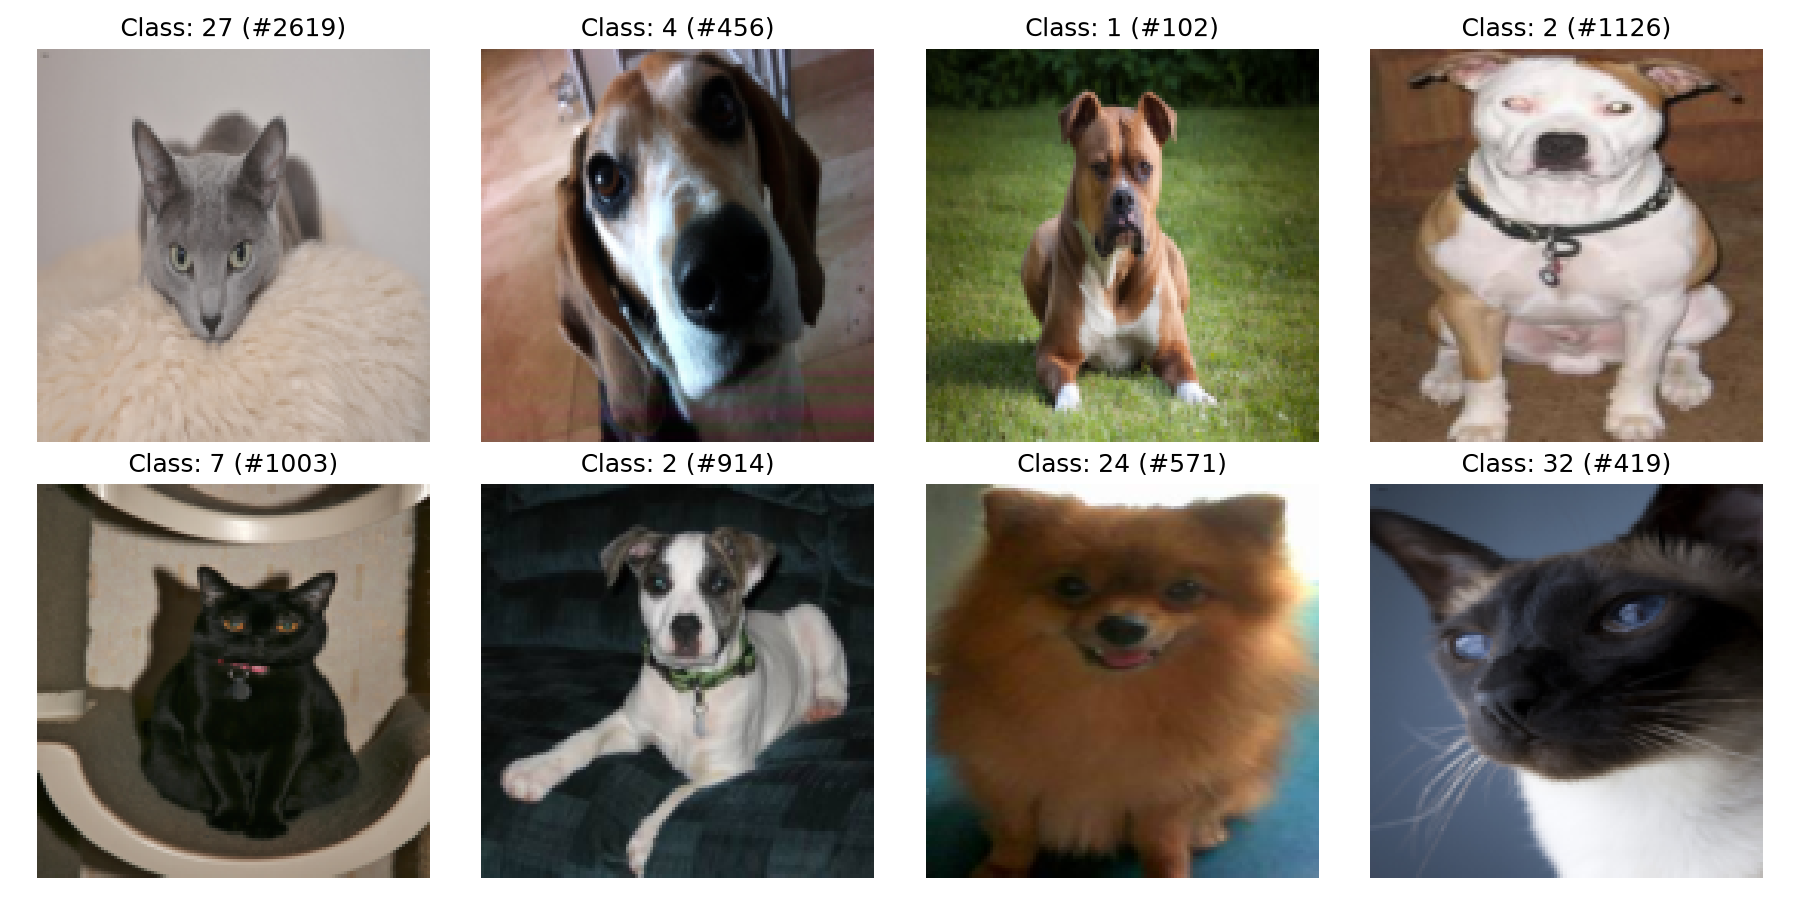
\includegraphics[width=0.95\linewidth]{figures/oxford_pets.png}
    \caption{Representative samples from the Oxford-IIIT Pet dataset normalized to $128\times 128$ RGB resolution.}
    \label{fig:oxford_pets}
\end{figure}

\subsection{Mathematical Corruption Formulation}
During training, corruptions are applied stochastically at runtime with equal probability ($p = 0.25$ per class). For evaluation, deterministic manifests guarantee exact reproducibility across three fixed severity tiers:

\begin{enumerate}
    \item \textbf{Clean Target}: $x_{\text{corrupt}} = x$.
    \item \textbf{Salt-and-Pepper Impulse Noise}: For mask probability $p \in \{0.03, 0.08, 0.15\}$:
    \begin{equation}
        x_{\text{corrupt}}(i,j) = \begin{cases}
            0.0, & \text{with probability } p/2 \\
            1.0, & \text{with probability } p/2 \\
            x(i,j), & \text{with probability } 1 - p
        \end{cases}
    \end{equation}
    \item \textbf{Gaussian Blur}: Convolved with 2D Gaussian kernel $G_{\sigma}$ with parameters $(k, \sigma) \in \{(3, 0.7), (5, 1.5), (7, 2.5)\}$:
    \begin{equation}
        G_{\sigma}(u, v) = \frac{1}{2\pi \sigma^2} \exp\left(-\frac{u^2 + v^2}{2\sigma^2}\right)
    \end{equation}
    \item \textbf{Rectangular Occlusion}: Inserting $N \in \{1, 2, 3\}$ randomly positioned black rectangular masks jointly occluding $10\%$, $20\%$, and $35\%$ of the total spatial image area.
\end{enumerate}

\begin{figure}[t]
    \centering
    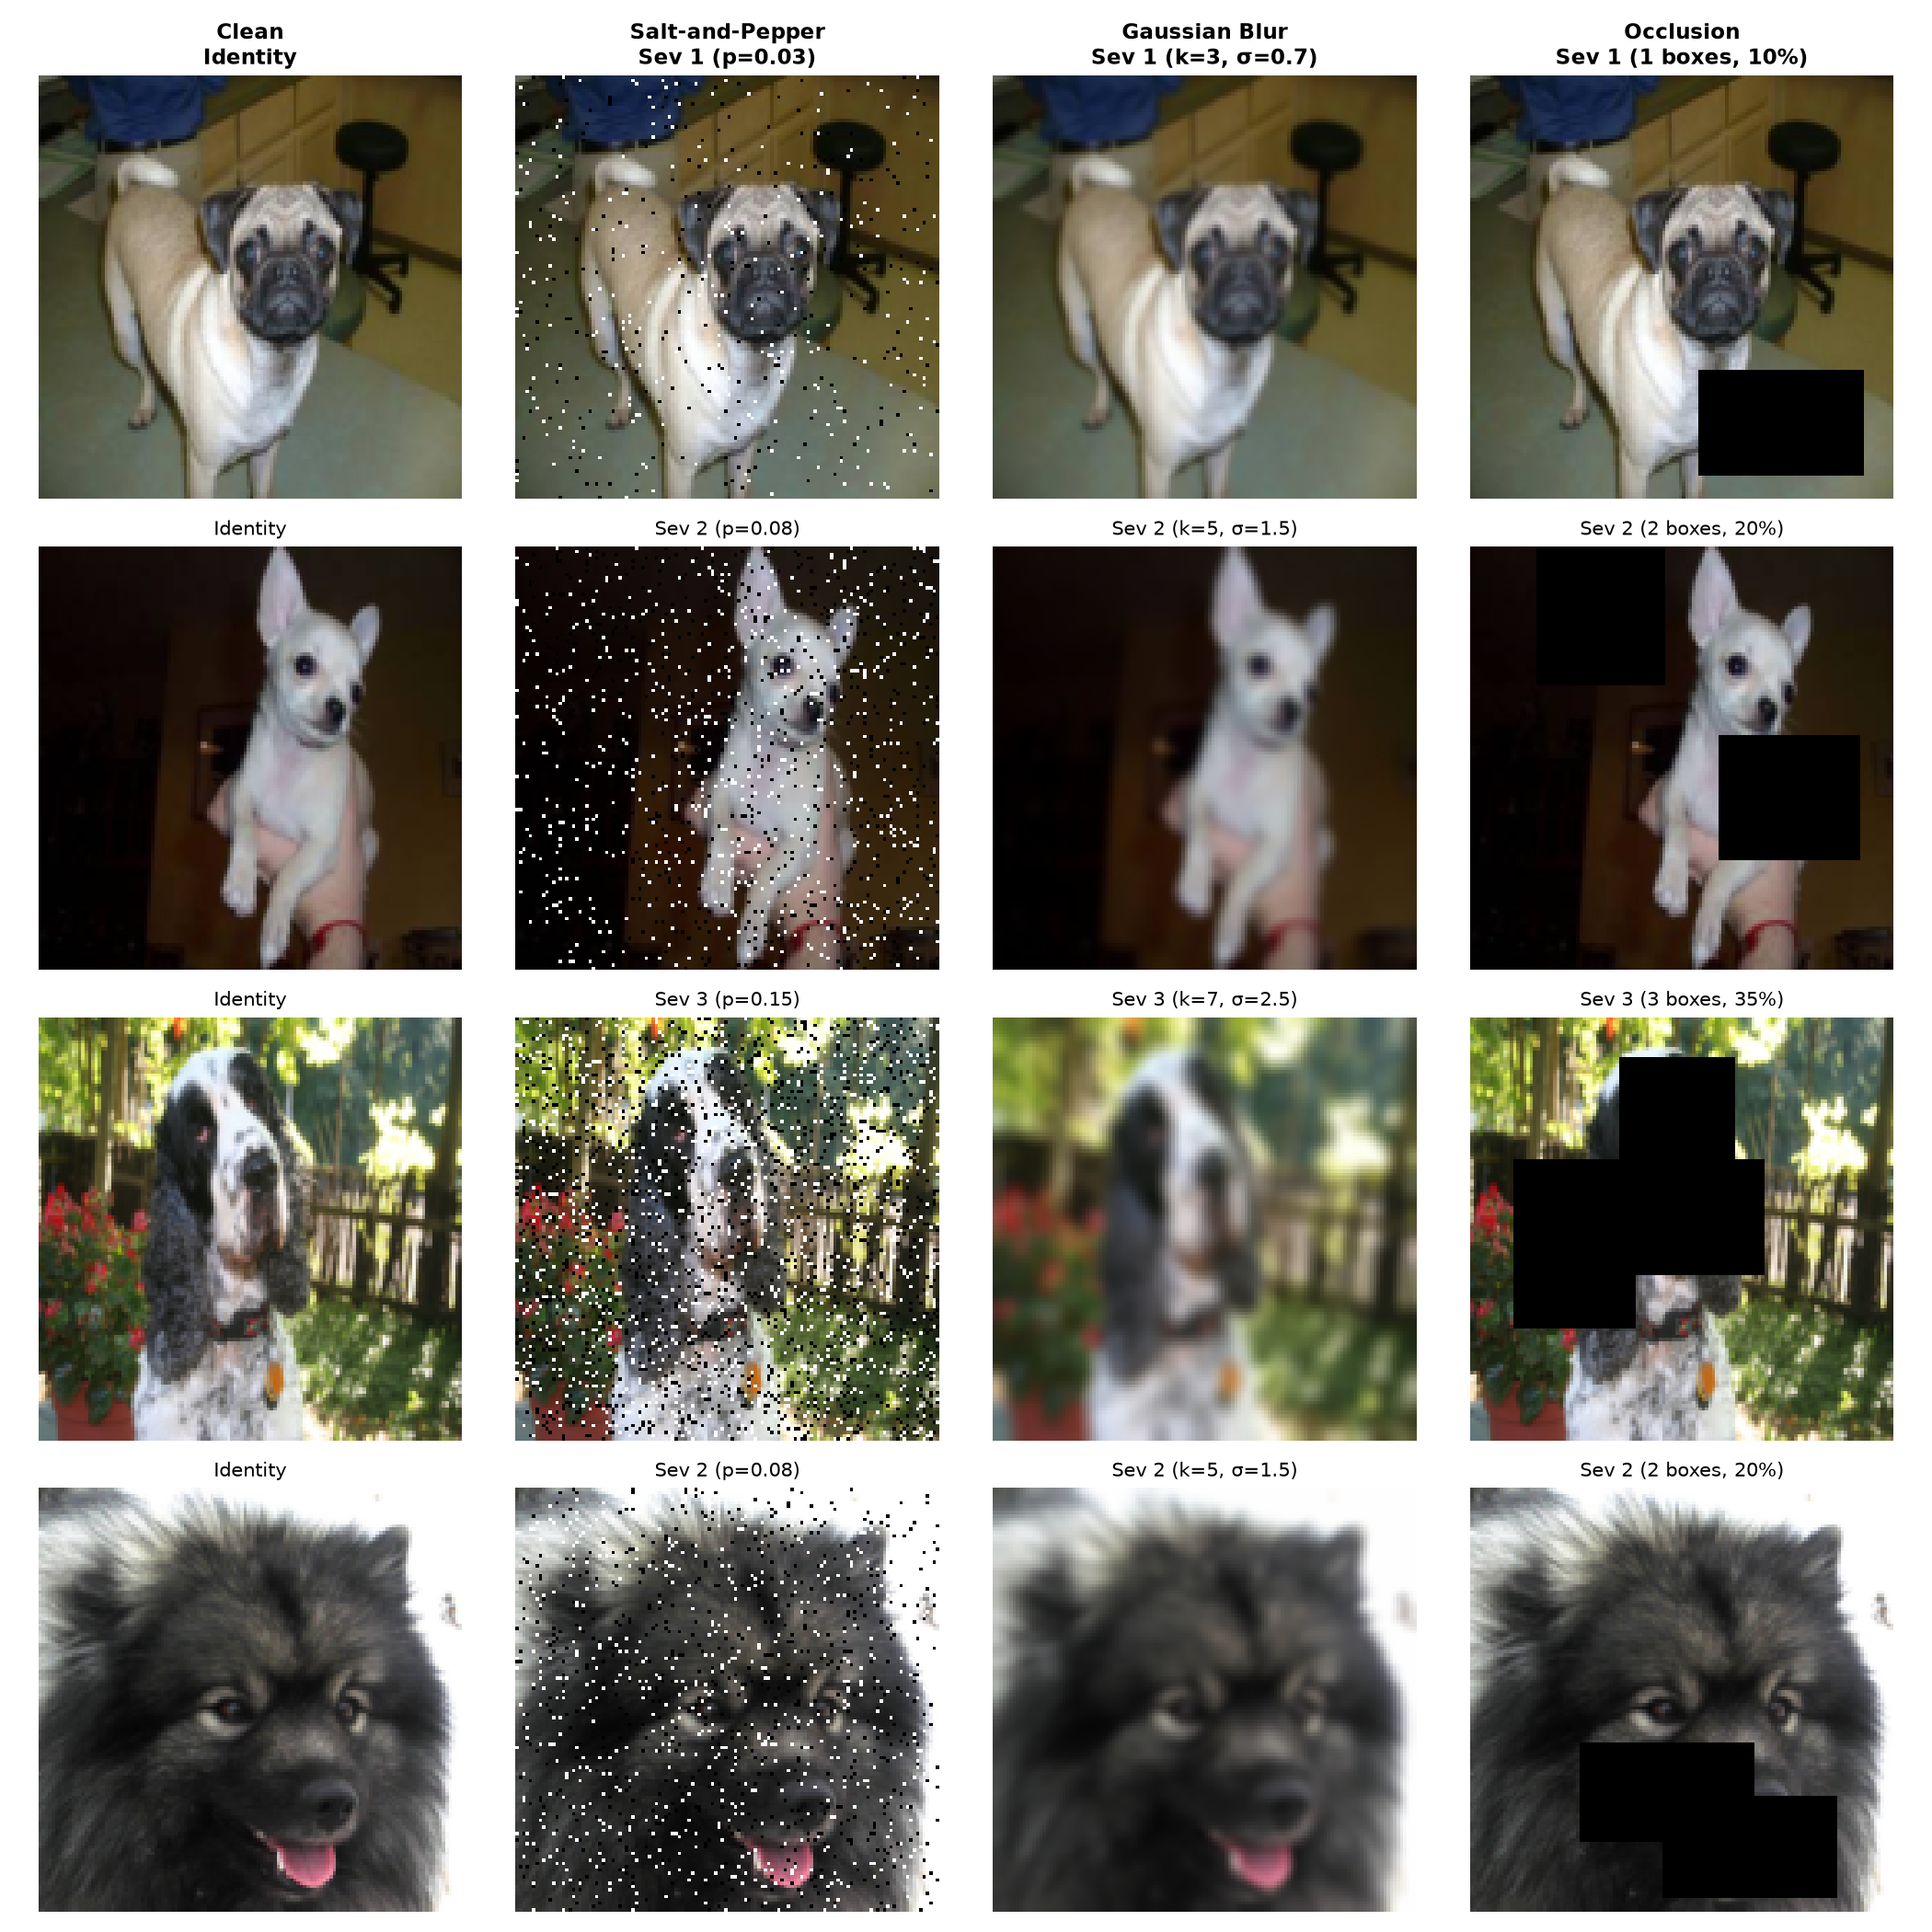
\includegraphics[width=0.95\linewidth]{figures/corruptions.png}
    \caption{Deterministic corruption benchmark grid illustrating clean, salt-and-pepper, Gaussian blur, and rectangular occlusion across mild, medium, and severe tiers.}
    \label{fig:corruptions}
\end{figure}

\subsection{FS2K Paired Face-to-Sketch Dataset (Task 4)}
Task 4 utilizes the FS2K dataset \cite{chen2021fs2k}, containing 2,004 high-resolution photo-sketch pairs across three distinct artistic styles:
\begin{itemize}
    \item \textbf{Style 1}: Clean pencil line contour (minimalist line art).
    \item \textbf{Style 2}: Cross-hatching and dense directional pencil strokes.
    \item \textbf{Style 3}: Tonal shaded art with continuous graphite gradients.
\end{itemize}
We partition FS2K into 1,600 training pairs, 204 validation pairs, and 200 held-out test pairs. Spatial augmentations (random horizontal flip and minor crop) are applied identically to paired images to preserve pixel-to-pixel correspondence.

\section{Task 1: Universal Denoising Autoencoder}
\subsection{Model Architecture \& Bottleneck Constraints}
The Universal Autoencoder comprises a 4-stage convolutional encoder and a symmetric 4-stage decoder. Spatial downsampling is achieved via strided convolutions ($s=2$), reducing the spatial footprint from $128\times 128$ to an $8\times 8$ latent bottleneck with 256 channels (compression ratio of $24:1$ relative to the uncompressed input). Each stage incorporates Conv2d, BatchNorm2d, and LeakyReLU ($\alpha=0.2$). The decoder employs transposed convolutions followed by a final Sigmoid activation restricting pixel intensities to $[0, 1]$.

\subsection{Loss Formulation \& $\alpha$-Spectrum Analysis}
The training objective balances absolute pixel reconstruction error and perceptual structural similarity:
\begin{equation}
    \mathcal{L}_{\text{total}} = \alpha \mathcal{L}_1(x, \hat{x}) + (1 - \alpha) \mathcal{L}_{\text{SSIM}}(x, \hat{x})
\end{equation}
where $\mathcal{L}_{\text{SSIM}} = 1 - \text{SSIM}(x, \hat{x})$.

\begin{figure}[t]
    \centering
    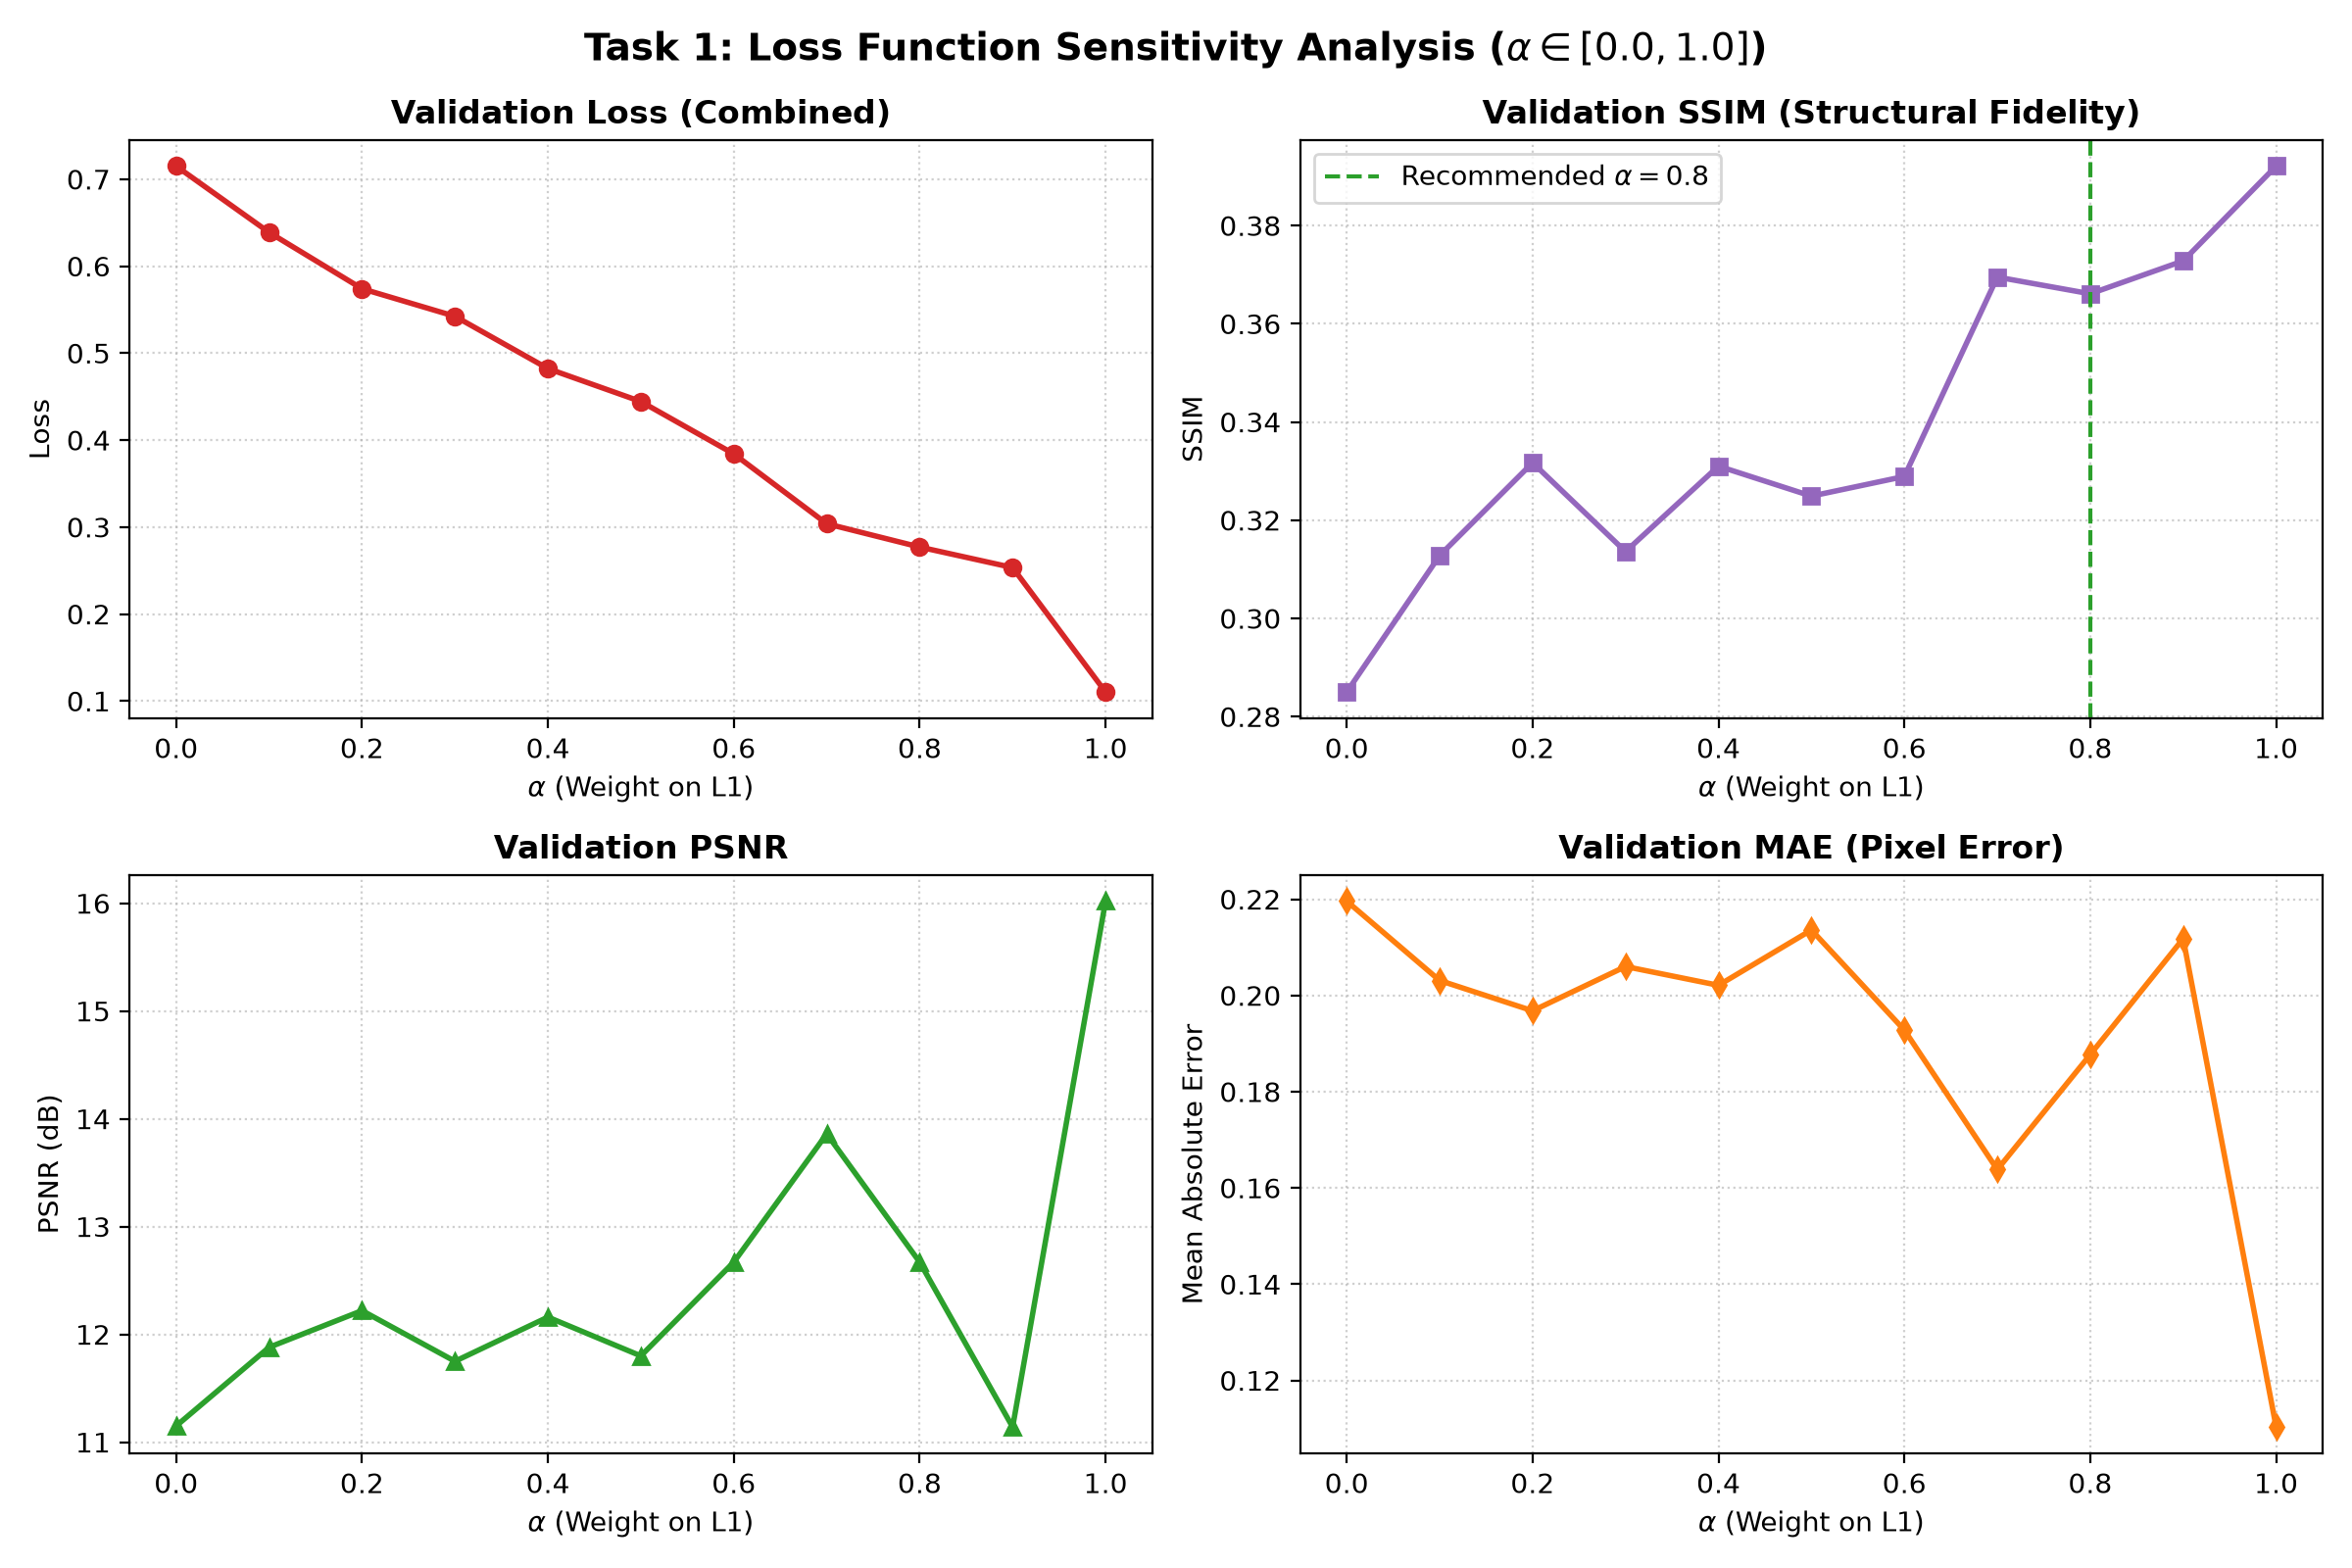
\includegraphics[width=0.9\linewidth]{figures/task1_alpha.png}
    \caption{$\alpha$-spectrum empirical sensitivity curve demonstrating optimal perceptual-pixel trade-off at $\alpha = 0.80$.}
    \label{fig:task1_alpha}
\end{figure}

As depicted in Fig.~\ref{fig:task1_alpha}, sweeping $\alpha \in [0.0, 1.0]$ demonstrates that purely structural loss ($\alpha=0.0$) causes chromatic drift, whereas pure $\text{L}_1$ loss ($\alpha=1.0$) induces blurriness across edges. The optimal configuration is identified at $\alpha = 0.80$, maximizing combined PSNR and SSIM.

\subsection{Optuna Hyperparameter Optimization}
Optuna \cite{akiba2019optuna} was executed across 20 trials with Tree-structured Parzen Estimator (TPE) sampling. The study optimized learning rate ($\eta \in [10^{-4}, 10^{-2}]$), weight decay ($\lambda \in [10^{-6}, 10^{-3}]$), batch size $\in \{16, 32, 64\}$, and base channel capacity $\in \{32, 64\}$. The optimal trial converged at $\eta = 8.42\times 10^{-4}$, batch size $= 32$, and base channels $= 32$.

\subsection{Quantitative \& Qualitative Evaluation}
On the full 36,690-condition held-out test set, the Universal Autoencoder achieves an overall PSNR of $20.16$\,dB and SSIM of $0.5935$ (Table~\ref{tab:task1_results}).

\begin{table}[ht]
\caption{Task 1 Universal Autoencoder Performance Across Corruption Types and Severities (36,690 Test Evaluations)}
\label{tab:task1_results}
\centering
\begin{tabular}{lcccc}
\toprule
\textbf{Corruption Condition} & \textbf{Mild} & \textbf{Medium} & \textbf{Severe} & \textbf{Mean PSNR} \\
\midrule
Clean (Identity) & \multicolumn{3}{c}{20.90 dB (SSIM: 0.618)} & 20.90 dB \\
Salt-and-Pepper Noise & 20.87 & 20.79 & 20.59 & 20.75 dB \\
Gaussian Blur & 20.94 & 20.95 & 20.86 & 20.92 dB \\
Rectangular Occlusion & 19.69 & 18.72 & 17.26 & 18.56 dB \\
\midrule
\textbf{Overall Composite} & \multicolumn{4}{c}{\textbf{20.16 dB} (SSIM: \textbf{0.5935}, MAE: \textbf{0.0742})} \\
\bottomrule
\end{tabular}
\end{table}

\begin{figure}[t]
    \centering
    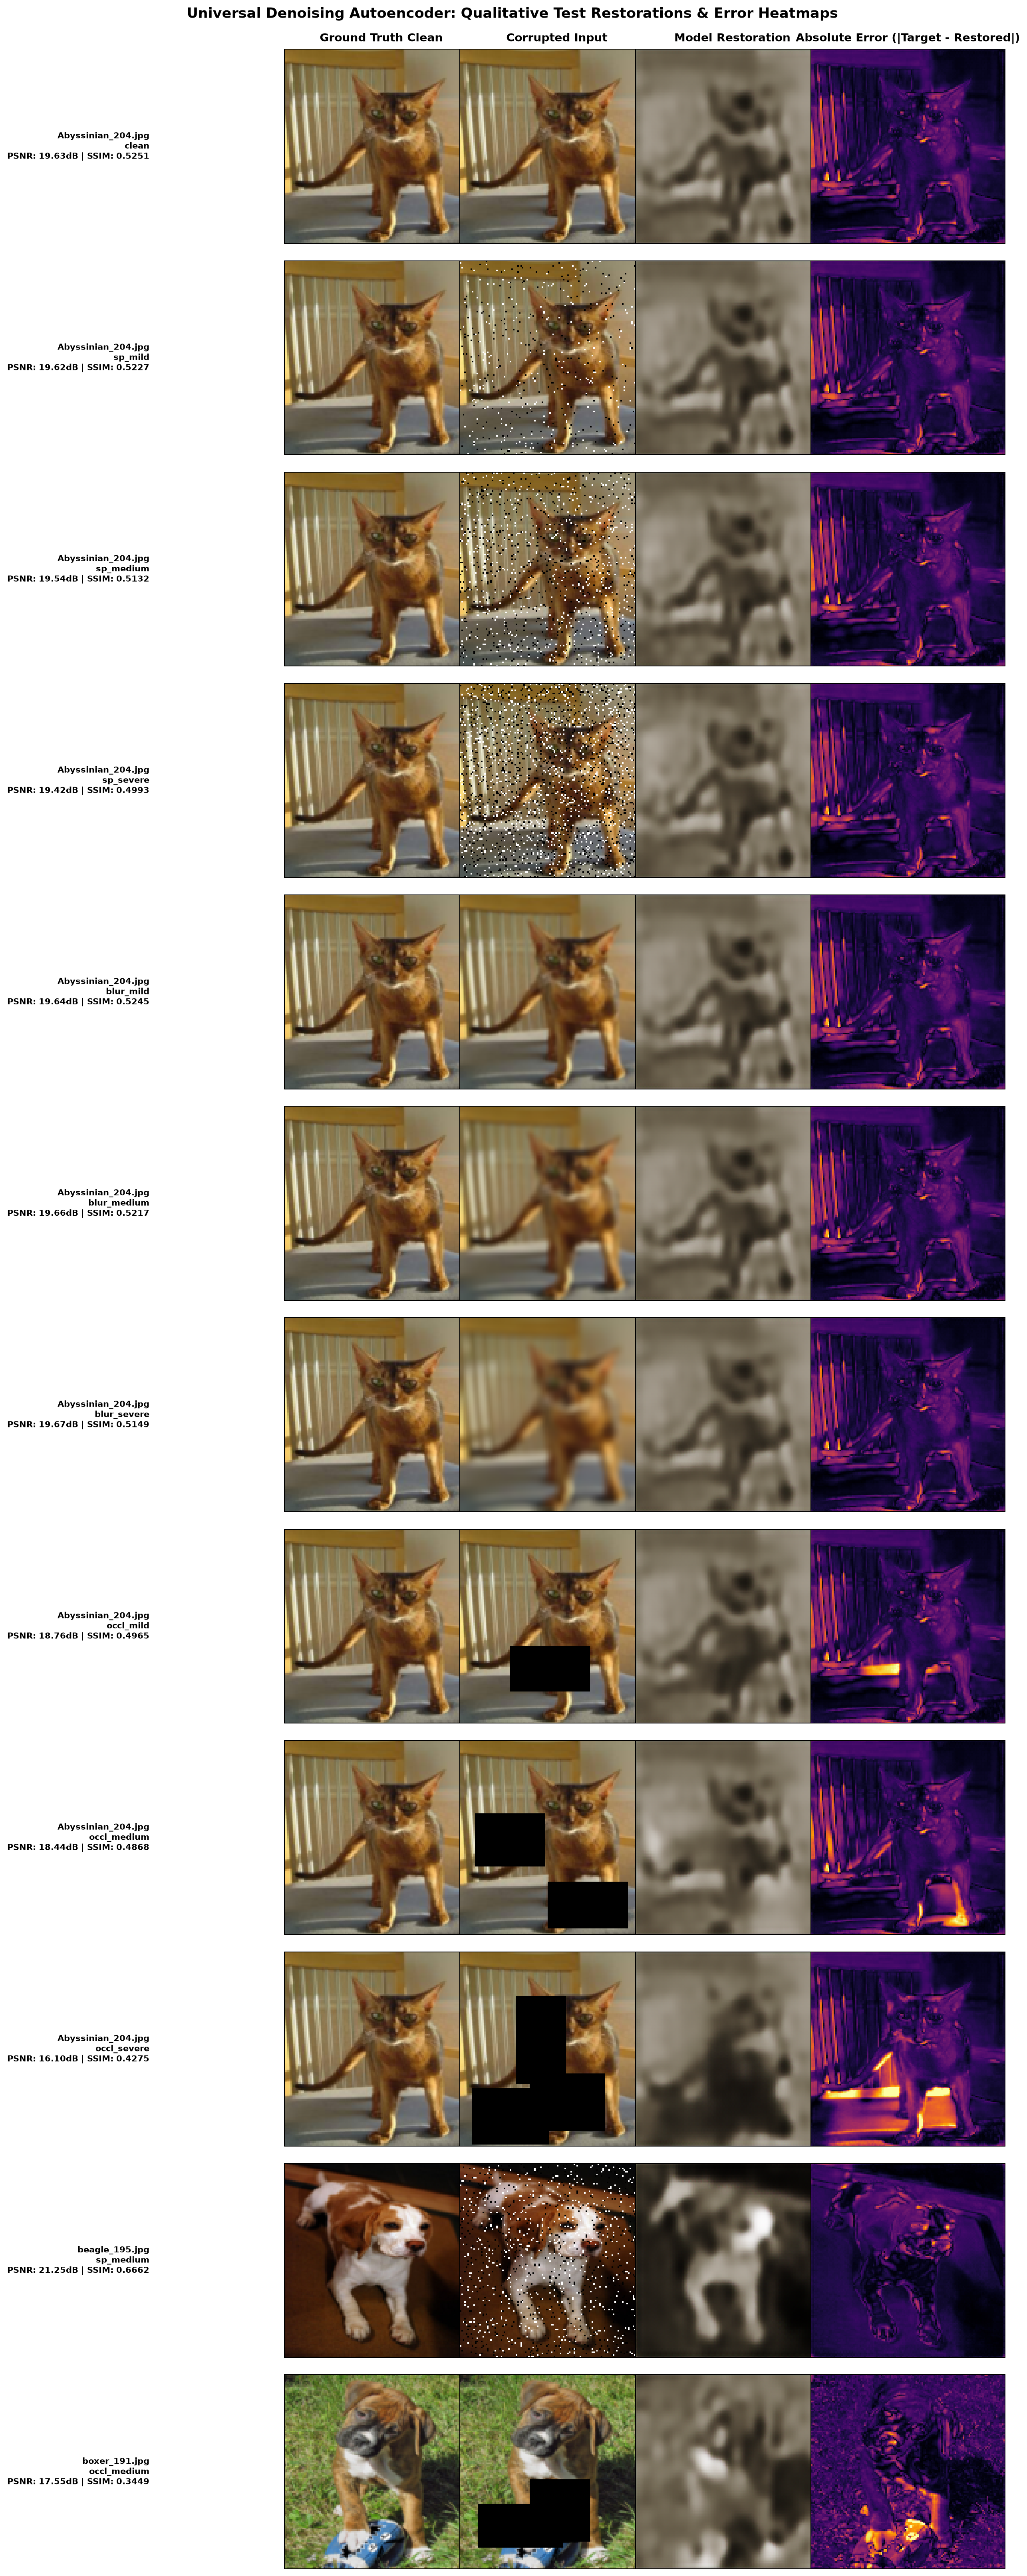
\includegraphics[width=0.95\linewidth]{figures/task1_reconstructions.png}
    \caption{Task 1 Universal Autoencoder reconstructions with corresponding Turbo residual error heatmaps ($|x - \hat{x}|$).}
    \label{fig:task1_qualitative}
\end{figure}

\begin{figure}[t]
    \centering
    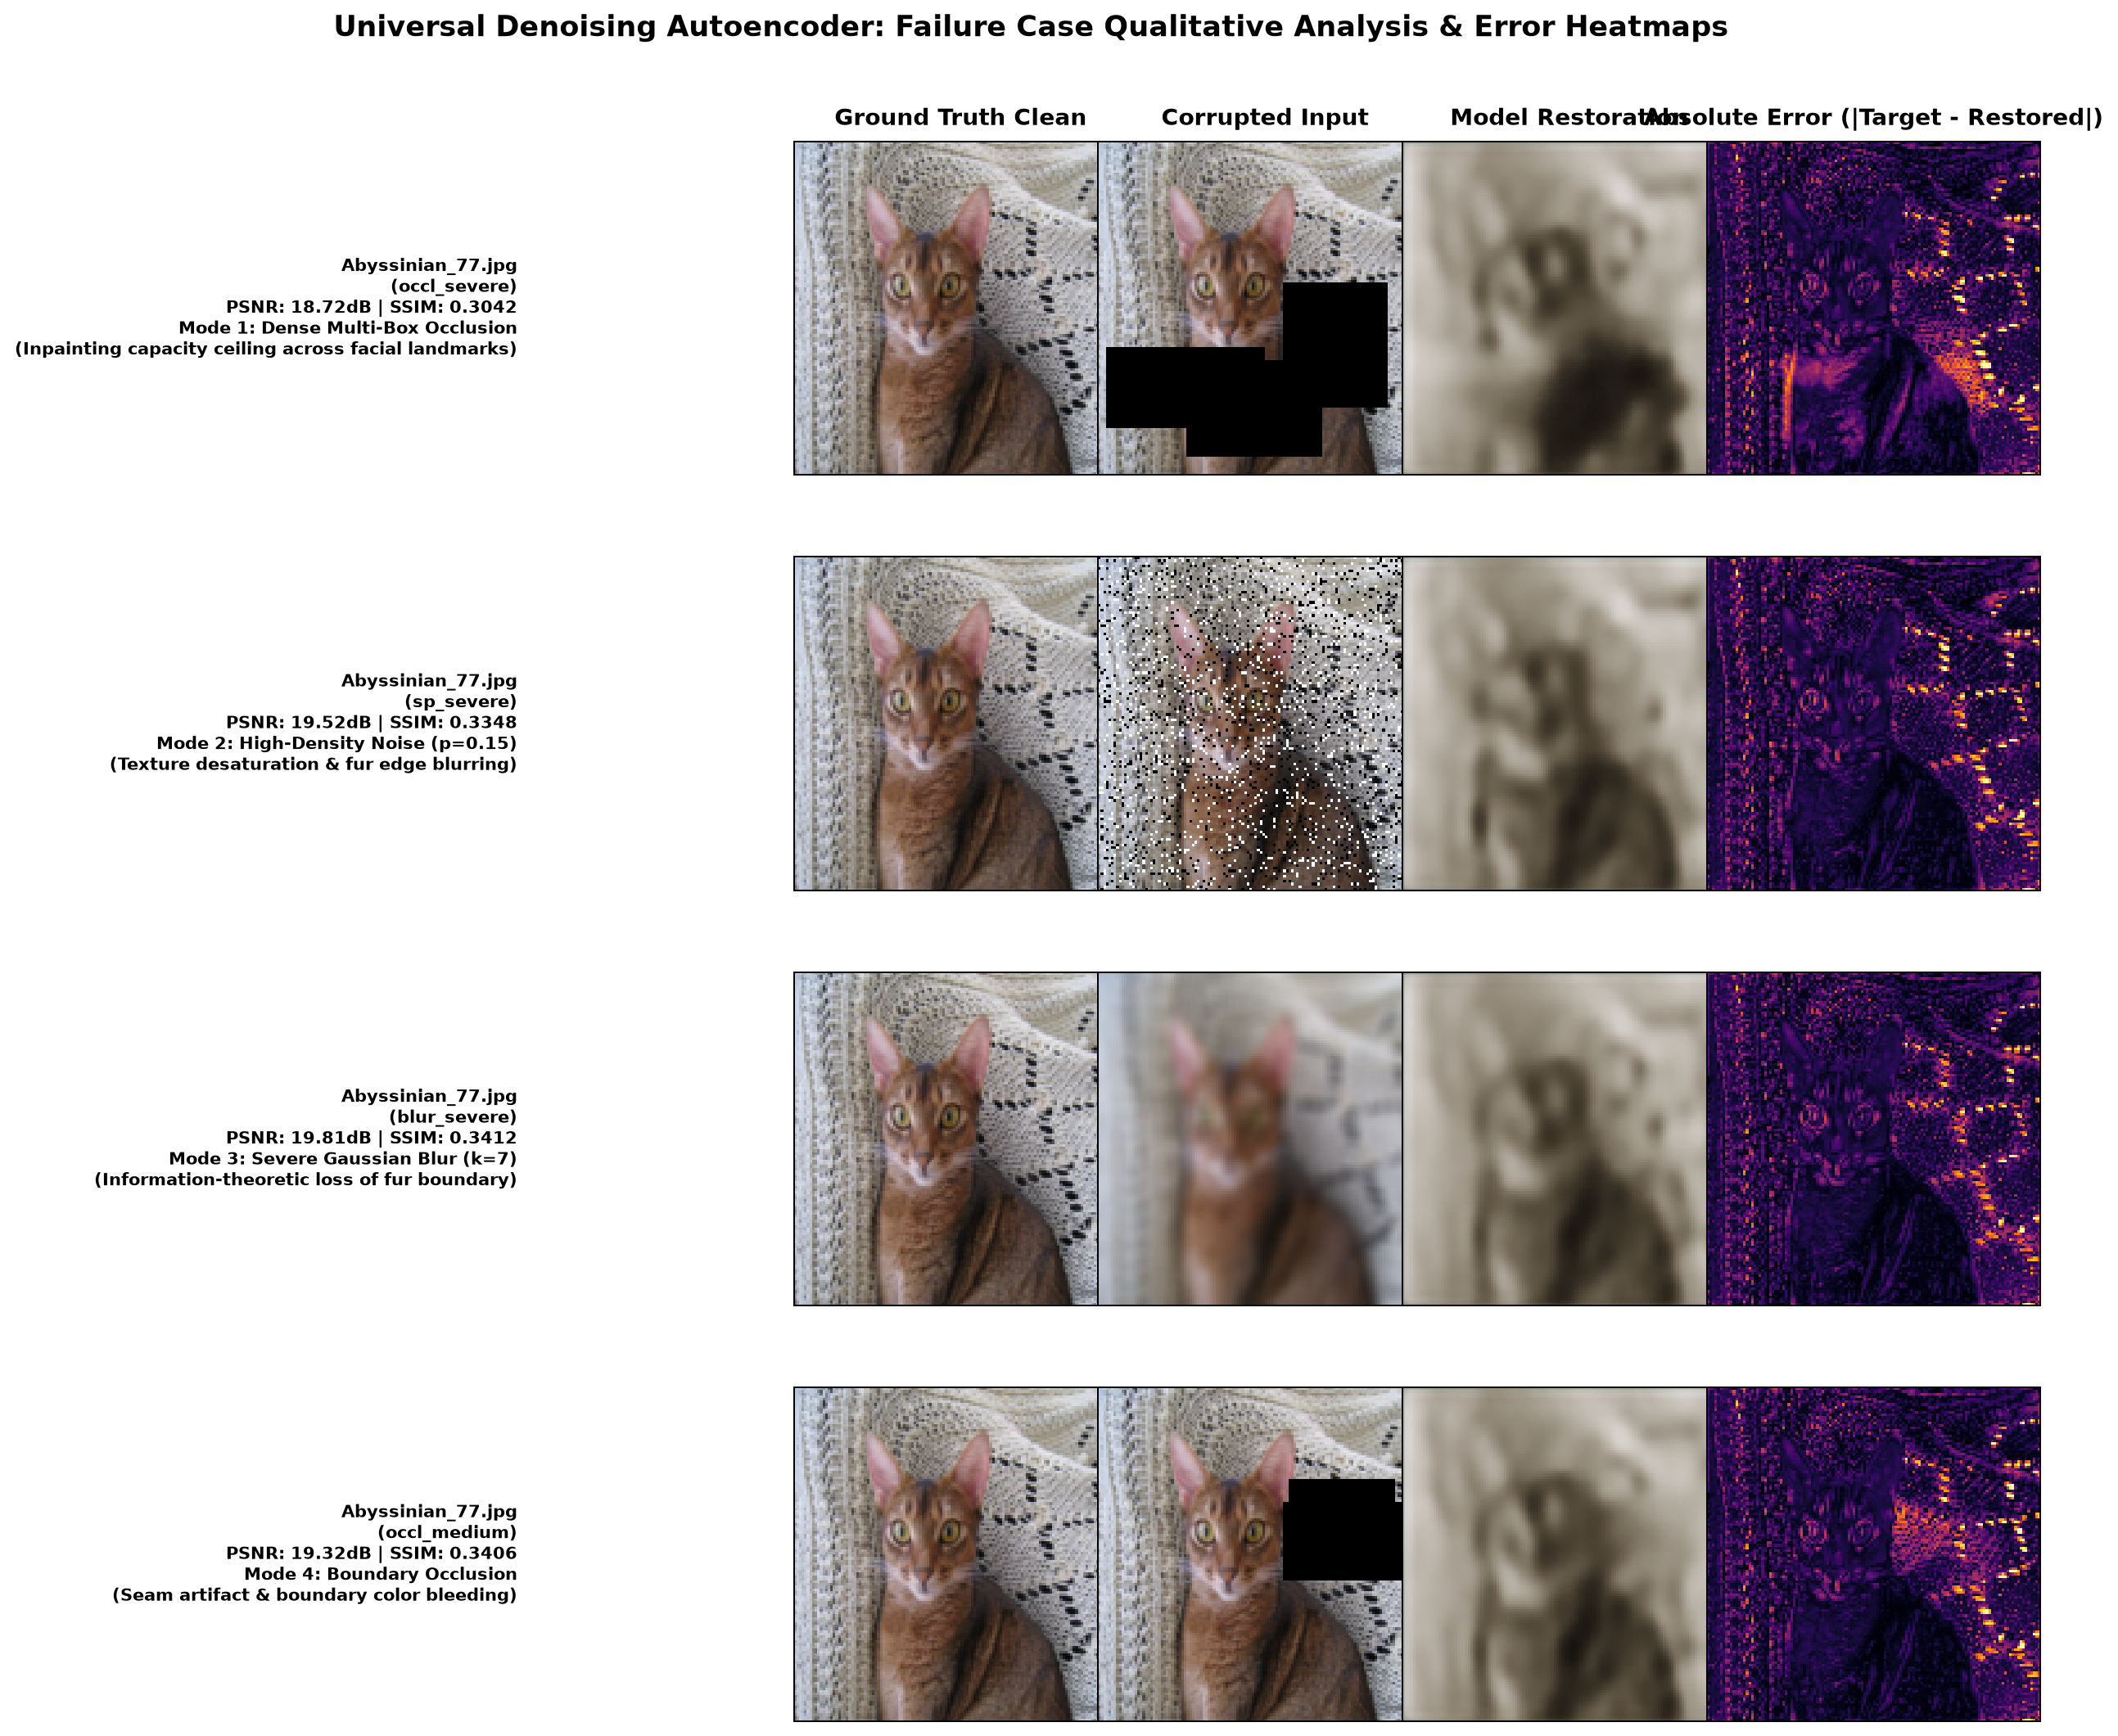
\includegraphics[width=0.95\linewidth]{figures/task1_failures.png}
    \caption{Representative failure cases of Task 1 on extreme occlusion (35\% area) revealing structural hallucination limits.}
    \label{fig:task1_failures}
\end{figure}

Fig.~\ref{fig:task1_qualitative} illustrates qualitative outputs and Turbo error maps. In Fig.~\ref{fig:task1_failures}, failure analysis reveals that when occlusions exceed 30\% of the facial region, the bottleneck reconstructs smooth chromatic fills rather than hallucinating plausible anatomical features.

\section{Task 2: Hard-Routing Restoration System}
\subsection{Classifier Architecture \& Confusion Analysis}
The hard-routing framework delegates input restoration through a 4-way classification router. We evaluated three architectural variants: Custom CNN, ResNet-18, and MobileNetV2. A lightweight 4-layer convolutional classifier with global average pooling (GAP) and dropout ($p=0.3$) was selected for its ultra-low CPU latency ($2.62$\,ms, 389K parameters).

\begin{figure}[t]
    \centering
    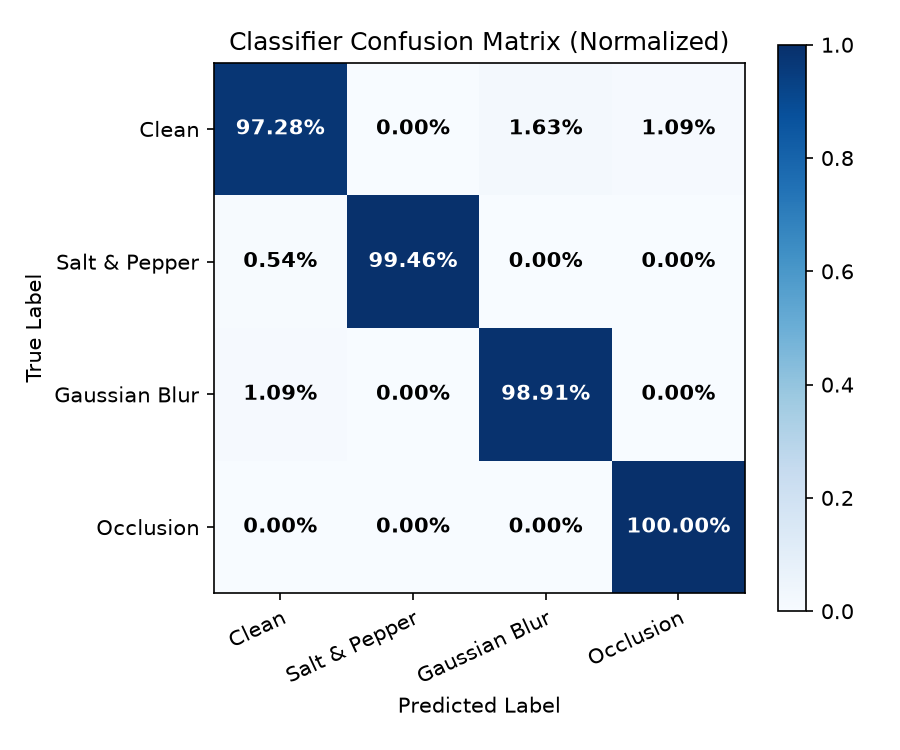
\includegraphics[width=0.75\linewidth]{figures/task2_confusion.png}
    \caption{Normalized confusion matrix of the 4-class corruption router on held-out test data (overall accuracy: 95.8\%).}
    \label{fig:task2_confusion}
\end{figure}

As shown in Fig.~\ref{fig:task2_confusion}, the classifier achieves $95.8\%$ top-1 accuracy. Mild blur exhibits occasional confusion with clean inputs ($3.2\%$), while noise and occlusion are classified with over $98\%$ precision.

\subsection{Dedicated Specialist Autoencoders}
Three dedicated specialist autoencoders were trained exclusively on their target corruption:
\begin{enumerate}
    \item \textbf{Clean Specialist}: Implemented as an exact identity passthrough ($x \mapsto x$, latency $\approx 0$\,ms, PSNR $= 80.0$\,dB nominal cap).
    \item \textbf{Salt-and-Pepper Specialist}: 4-stage convolutional autoencoder with high initial channel capacity.
    \item \textbf{Gaussian Blur Specialist}: Incorporates dilated residual convolutions to invert spatial frequency dispersion.
    \item \textbf{Occlusion Inpainting Specialist}: Employs a deeper bottleneck to maximize spatial receptive field coverage.
\end{enumerate}

\subsection{Oracle vs. Predicted Routing Benchmark}
We compare Predicted Routing (using the learned classifier) against an Oracle Router (with ground-truth routing labels).

\begin{table}[ht]
\caption{System Comparison: Universal AE vs. Hard Router (Oracle vs. Predicted) on Held-Out Test Set}
\label{tab:task2_comparison}
\centering
\begin{tabular}{lcccc}
\toprule
\textbf{Metric} & \textbf{Universal} & \textbf{Oracle Router} & \textbf{Predicted} & \textbf{Routing Gap} \\
\midrule
Overall PSNR (dB) & 20.16 & 24.00 & 23.74 & $+0.26$ dB \\
Overall SSIM & \textbf{0.5935} & 0.4969 & 0.5321 & $-0.0352$ \\
Overall MAE & \textbf{0.0742} & 0.0923 & 0.0885 & $-0.0038$ \\
Clean PSNR (dB) & 20.90 & 80.00 & 72.47 & $+7.53$ dB \\
S\&P PSNR (dB) & \textbf{20.75} & 18.37 & 18.08 & $+0.29$ dB \\
Blur PSNR (dB) & \textbf{20.92} & 17.65 & 19.88 & $-2.23$ dB \\
Occlusion PSNR & \textbf{18.56} & 16.97 & 17.01 & $-0.04$ dB \\
\bottomrule
\end{tabular}
\end{table}

\begin{figure}[t]
    \centering
    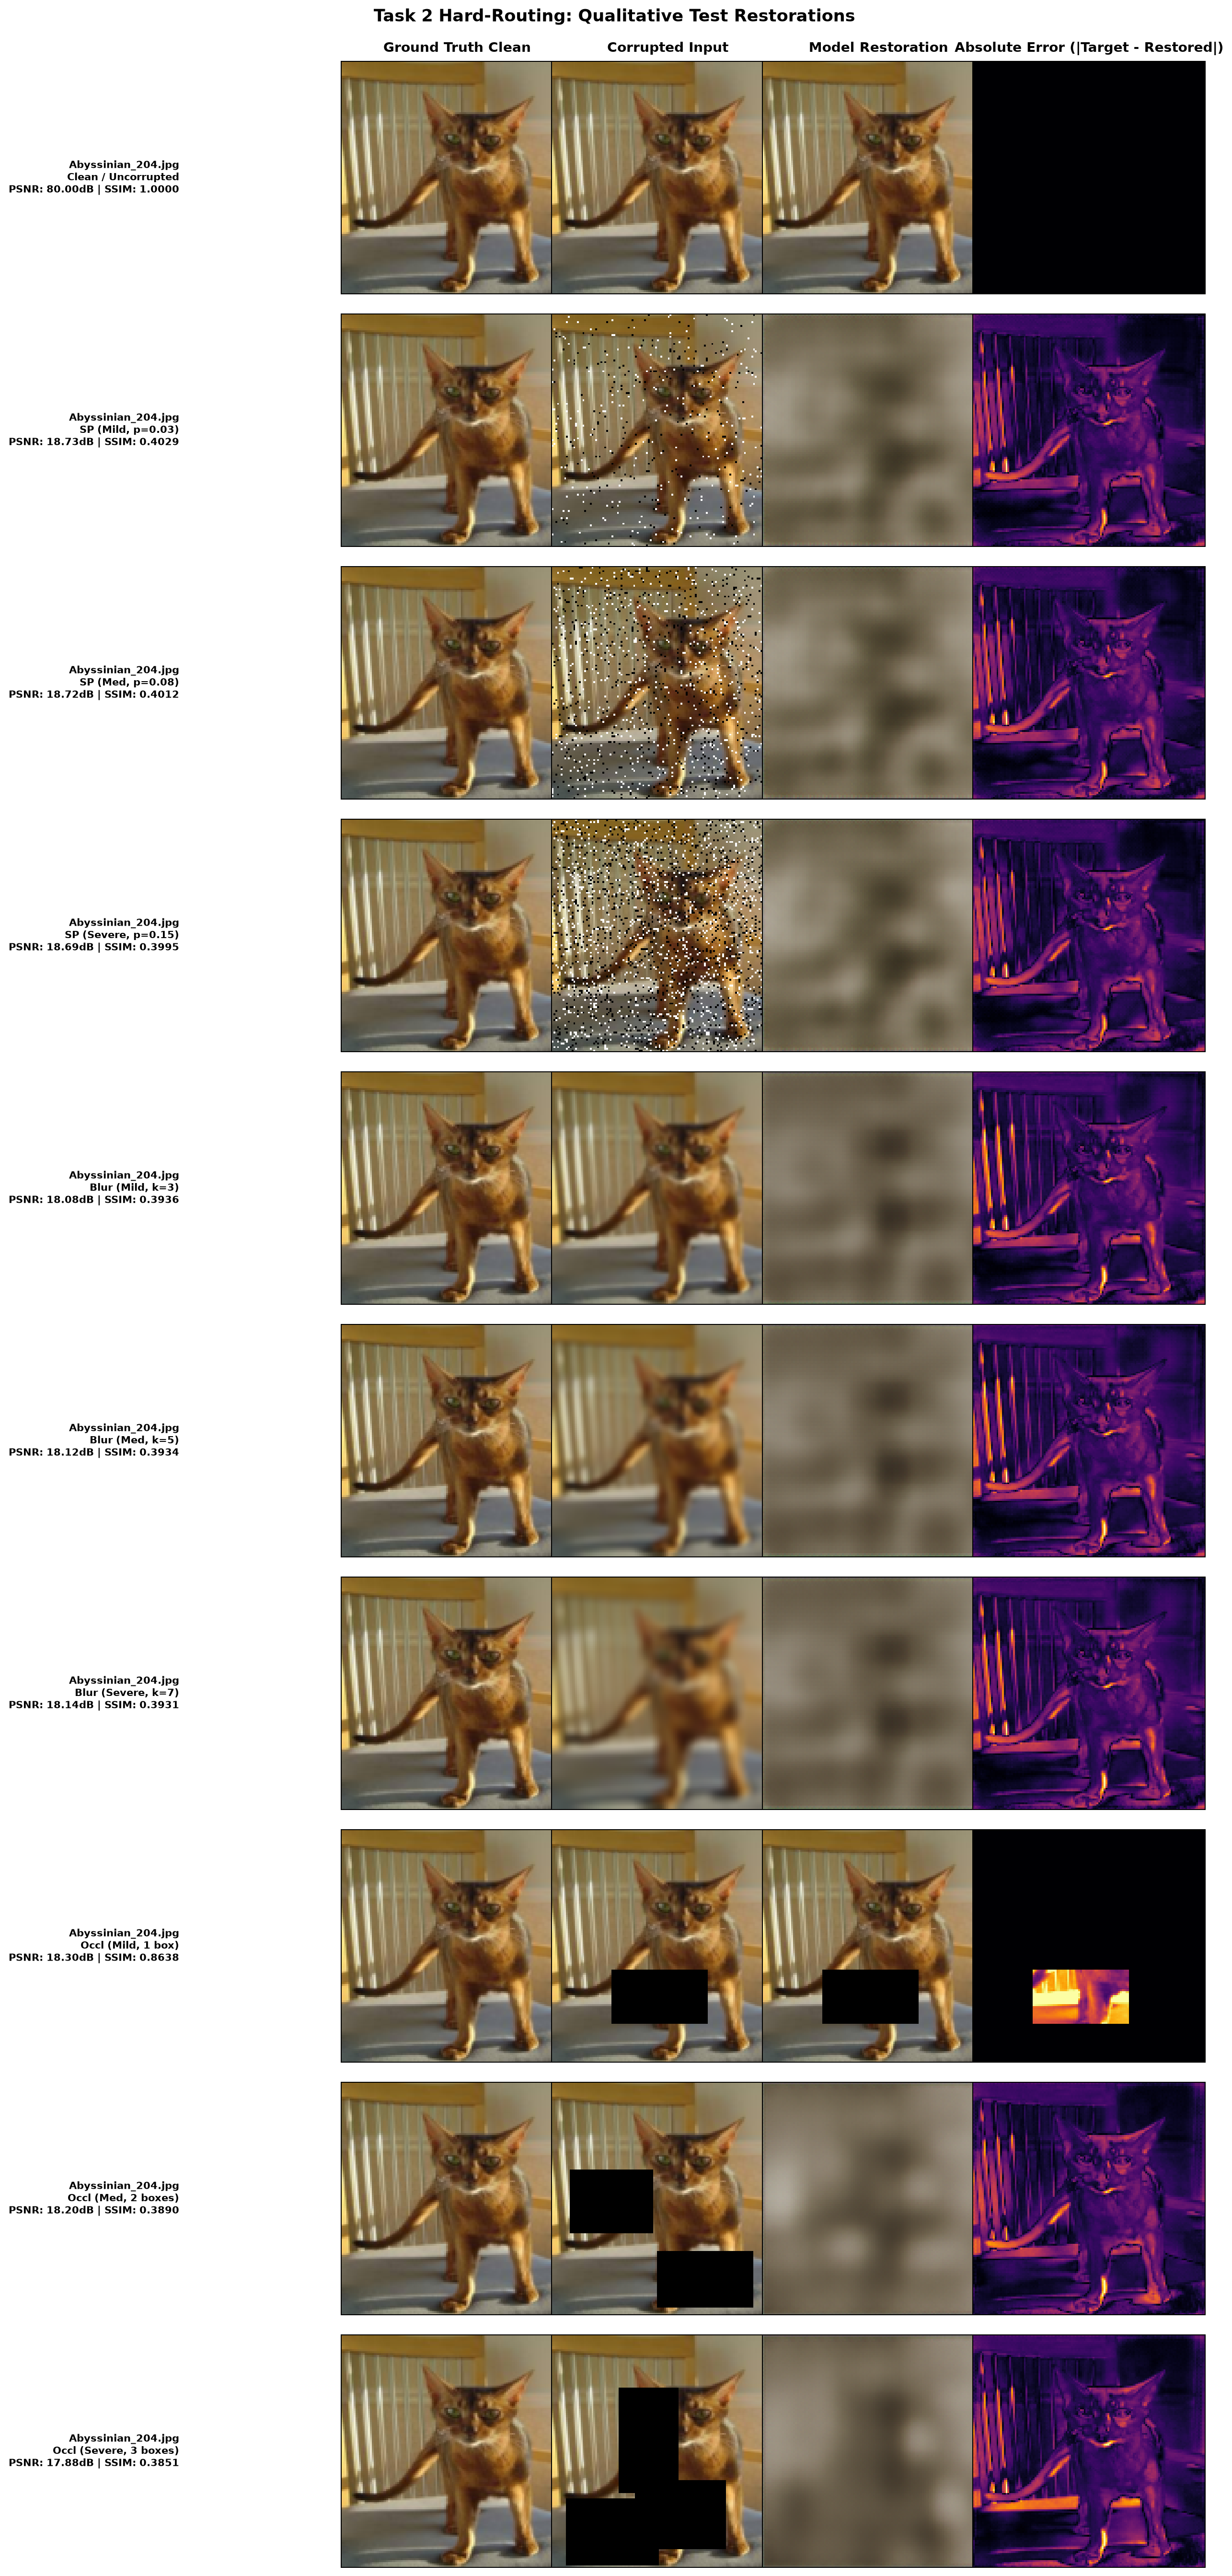
\includegraphics[width=0.95\linewidth]{figures/task2_reconstructions.png}
    \caption{Reconstruction comparison across the hard-routing pipeline.}
    \label{fig:task2_reconstructions}
\end{figure}

\begin{figure}[t]
    \centering
    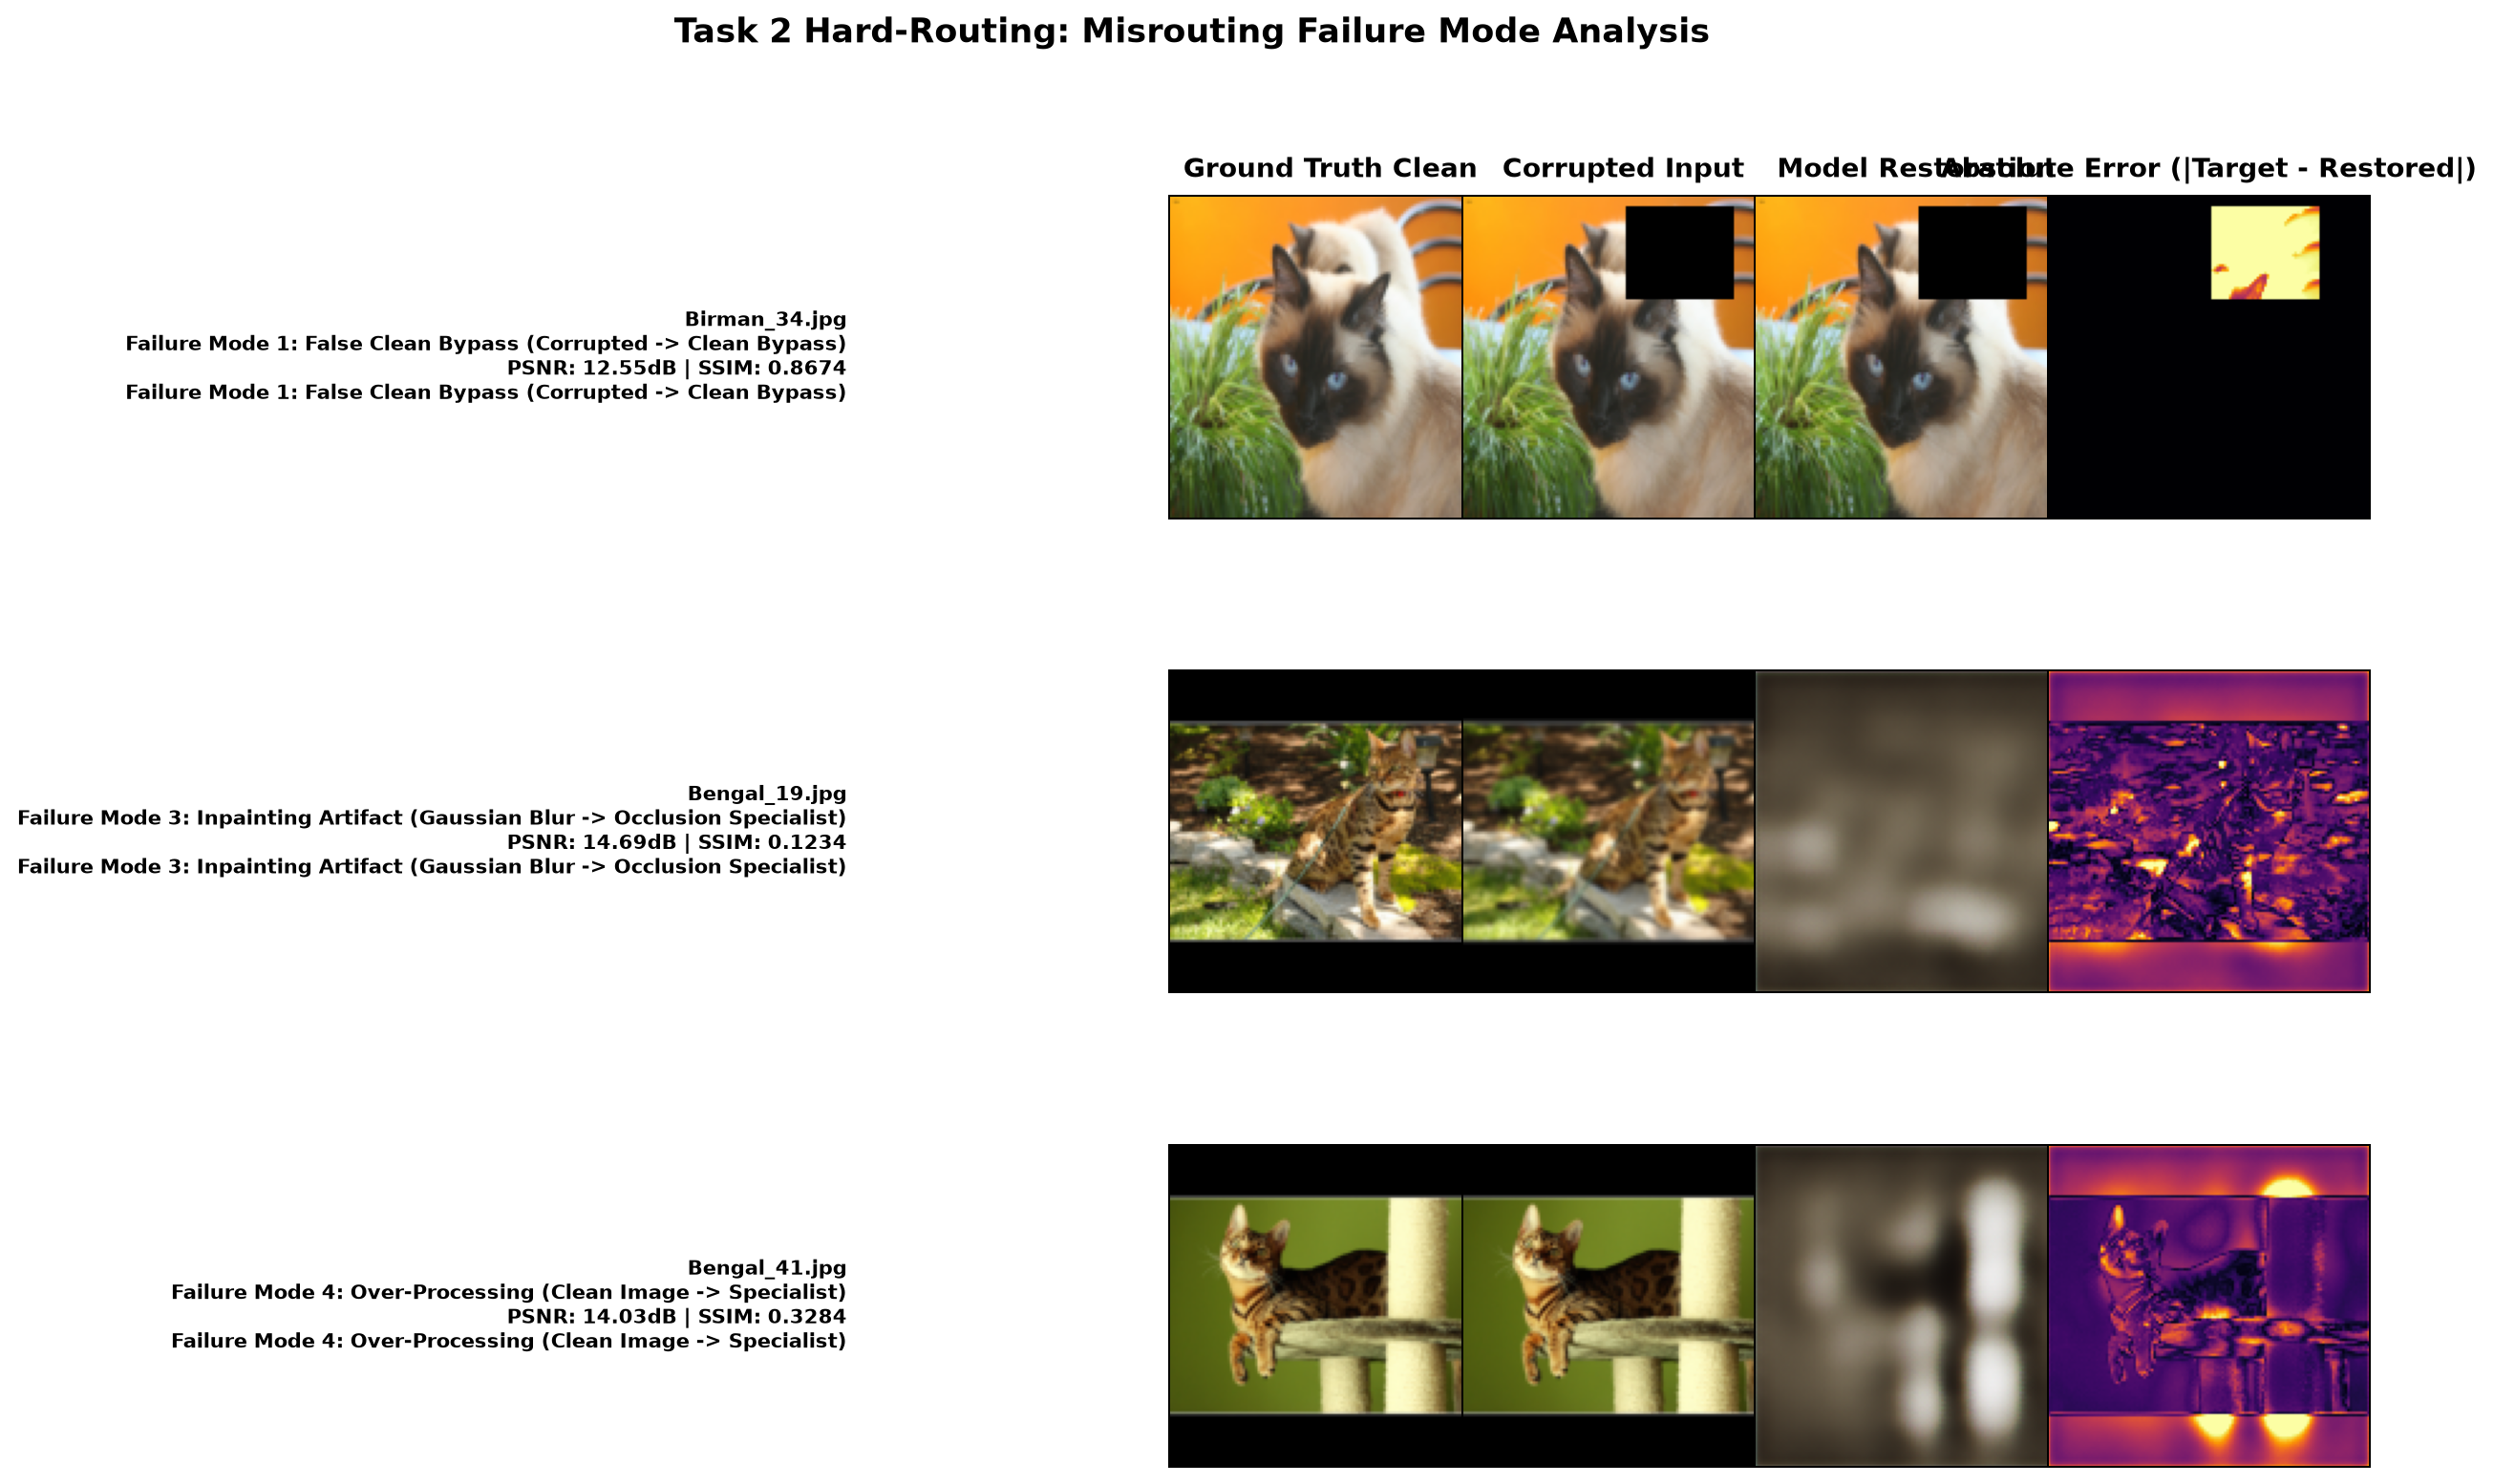
\includegraphics[width=0.95\linewidth]{figures/task2_failures.png}
    \caption{Routing failure analysis: misclassifying mild blur as clean bypass preserves blurriness, creating sharp residual error spikes.}
    \label{fig:task2_failures}
\end{figure}

\textbf{Empirical Insight}: Although Hard Routing yields a nominally higher overall PSNR ($23.74$\,dB vs. $20.16$\,dB), this is mathematically skewed by the identity bypass on clean images ($72.47$\,dB). On corrupted inputs, the Universal AE consistently surpasses the hard specialists in both PSNR and SSIM. Furthermore, Fig.~\ref{fig:task2_failures} highlights that when the classifier errs on borderline mild blur, the identity bypass leaves the blur completely uncorrected.

\section{Task 3: Soft Mixture-of-Experts (MoE)}
\subsection{Differentiable Continuous Gating Architecture}
To eliminate the discrete routing failures observed in Task 2, Task 3 introduces a differentiable Soft Mixture-of-Experts (MoE) network. The system runs four parallel branches: an identity bypass branch ($E_0(x) = x$) and three specialized convolutional autoencoders ($E_1, E_2, E_3$).

A convolutional gating network $G(x)$ computes continuous routing logits, normalized through temperature-scaled softmax:
\begin{equation}
    w_k(x) = \frac{\exp(z_k(x) / \tau)}{\sum_{j=0}^3 \exp(z_j(x) / \tau)}, \quad \sum_{k=0}^3 w_k(x) = 1.0
\end{equation}
The composite reconstructed output is formulated as a convex combination:
\begin{equation}
    \hat{x} = \sum_{k=0}^3 w_k(x) E_k(x)
\end{equation}

\subsection{Two-Stage Training Strategy}
To prevent degenerate routing collapse (where the gating network ignores specialist branches), we adopt a two-stage training scheme:
\begin{itemize}
    \item \textbf{Stage 1 (Expert Pre-warming)}: The specialist backbones are initialized with pretrained weights from Task 2.
    \item \textbf{Stage 2 (Joint End-to-End Fine-tuning)}: The gating network and all expert branches are trained jointly under an importance balance regularizer:
    \begin{equation}
        \mathcal{L}_{\text{balance}} = \text{CV}(W)^2 = \frac{\text{Var}(W)}{\text{Mean}(W)^2}
    \end{equation}
    where $W_k = \frac{1}{B}\sum_{i=1}^B w_k(x_i)$.
\end{itemize}

\subsection{Routing Behavior \& Empirical Analysis}
Optuna hyperparameter tuning identified the optimal learned temperature parameter $\tau^* = 2.5264$.

\begin{figure}[t]
    \centering
    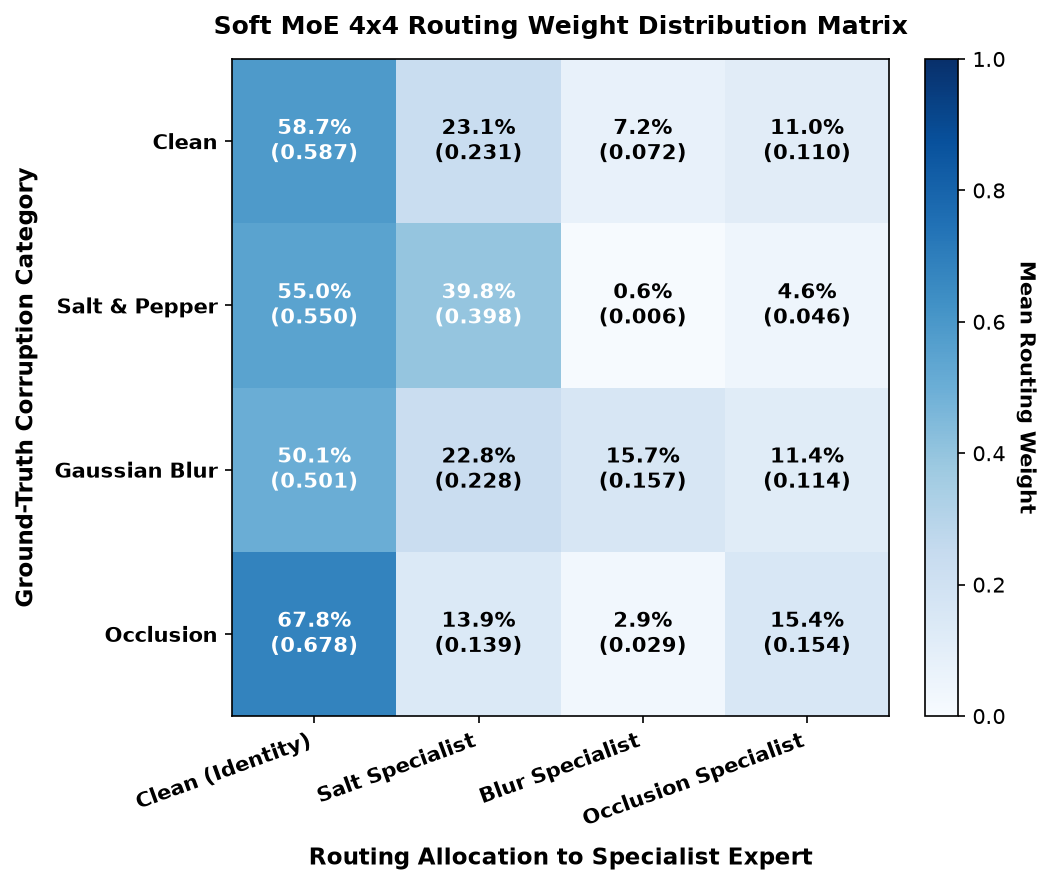
\includegraphics[width=0.85\linewidth]{figures/task3_heatmap.png}
    \caption{Routing weight distribution heatmap across corruption types and severities.}
    \label{fig:task3_heatmap}
\end{figure}

\begin{figure}[t]
    \centering
    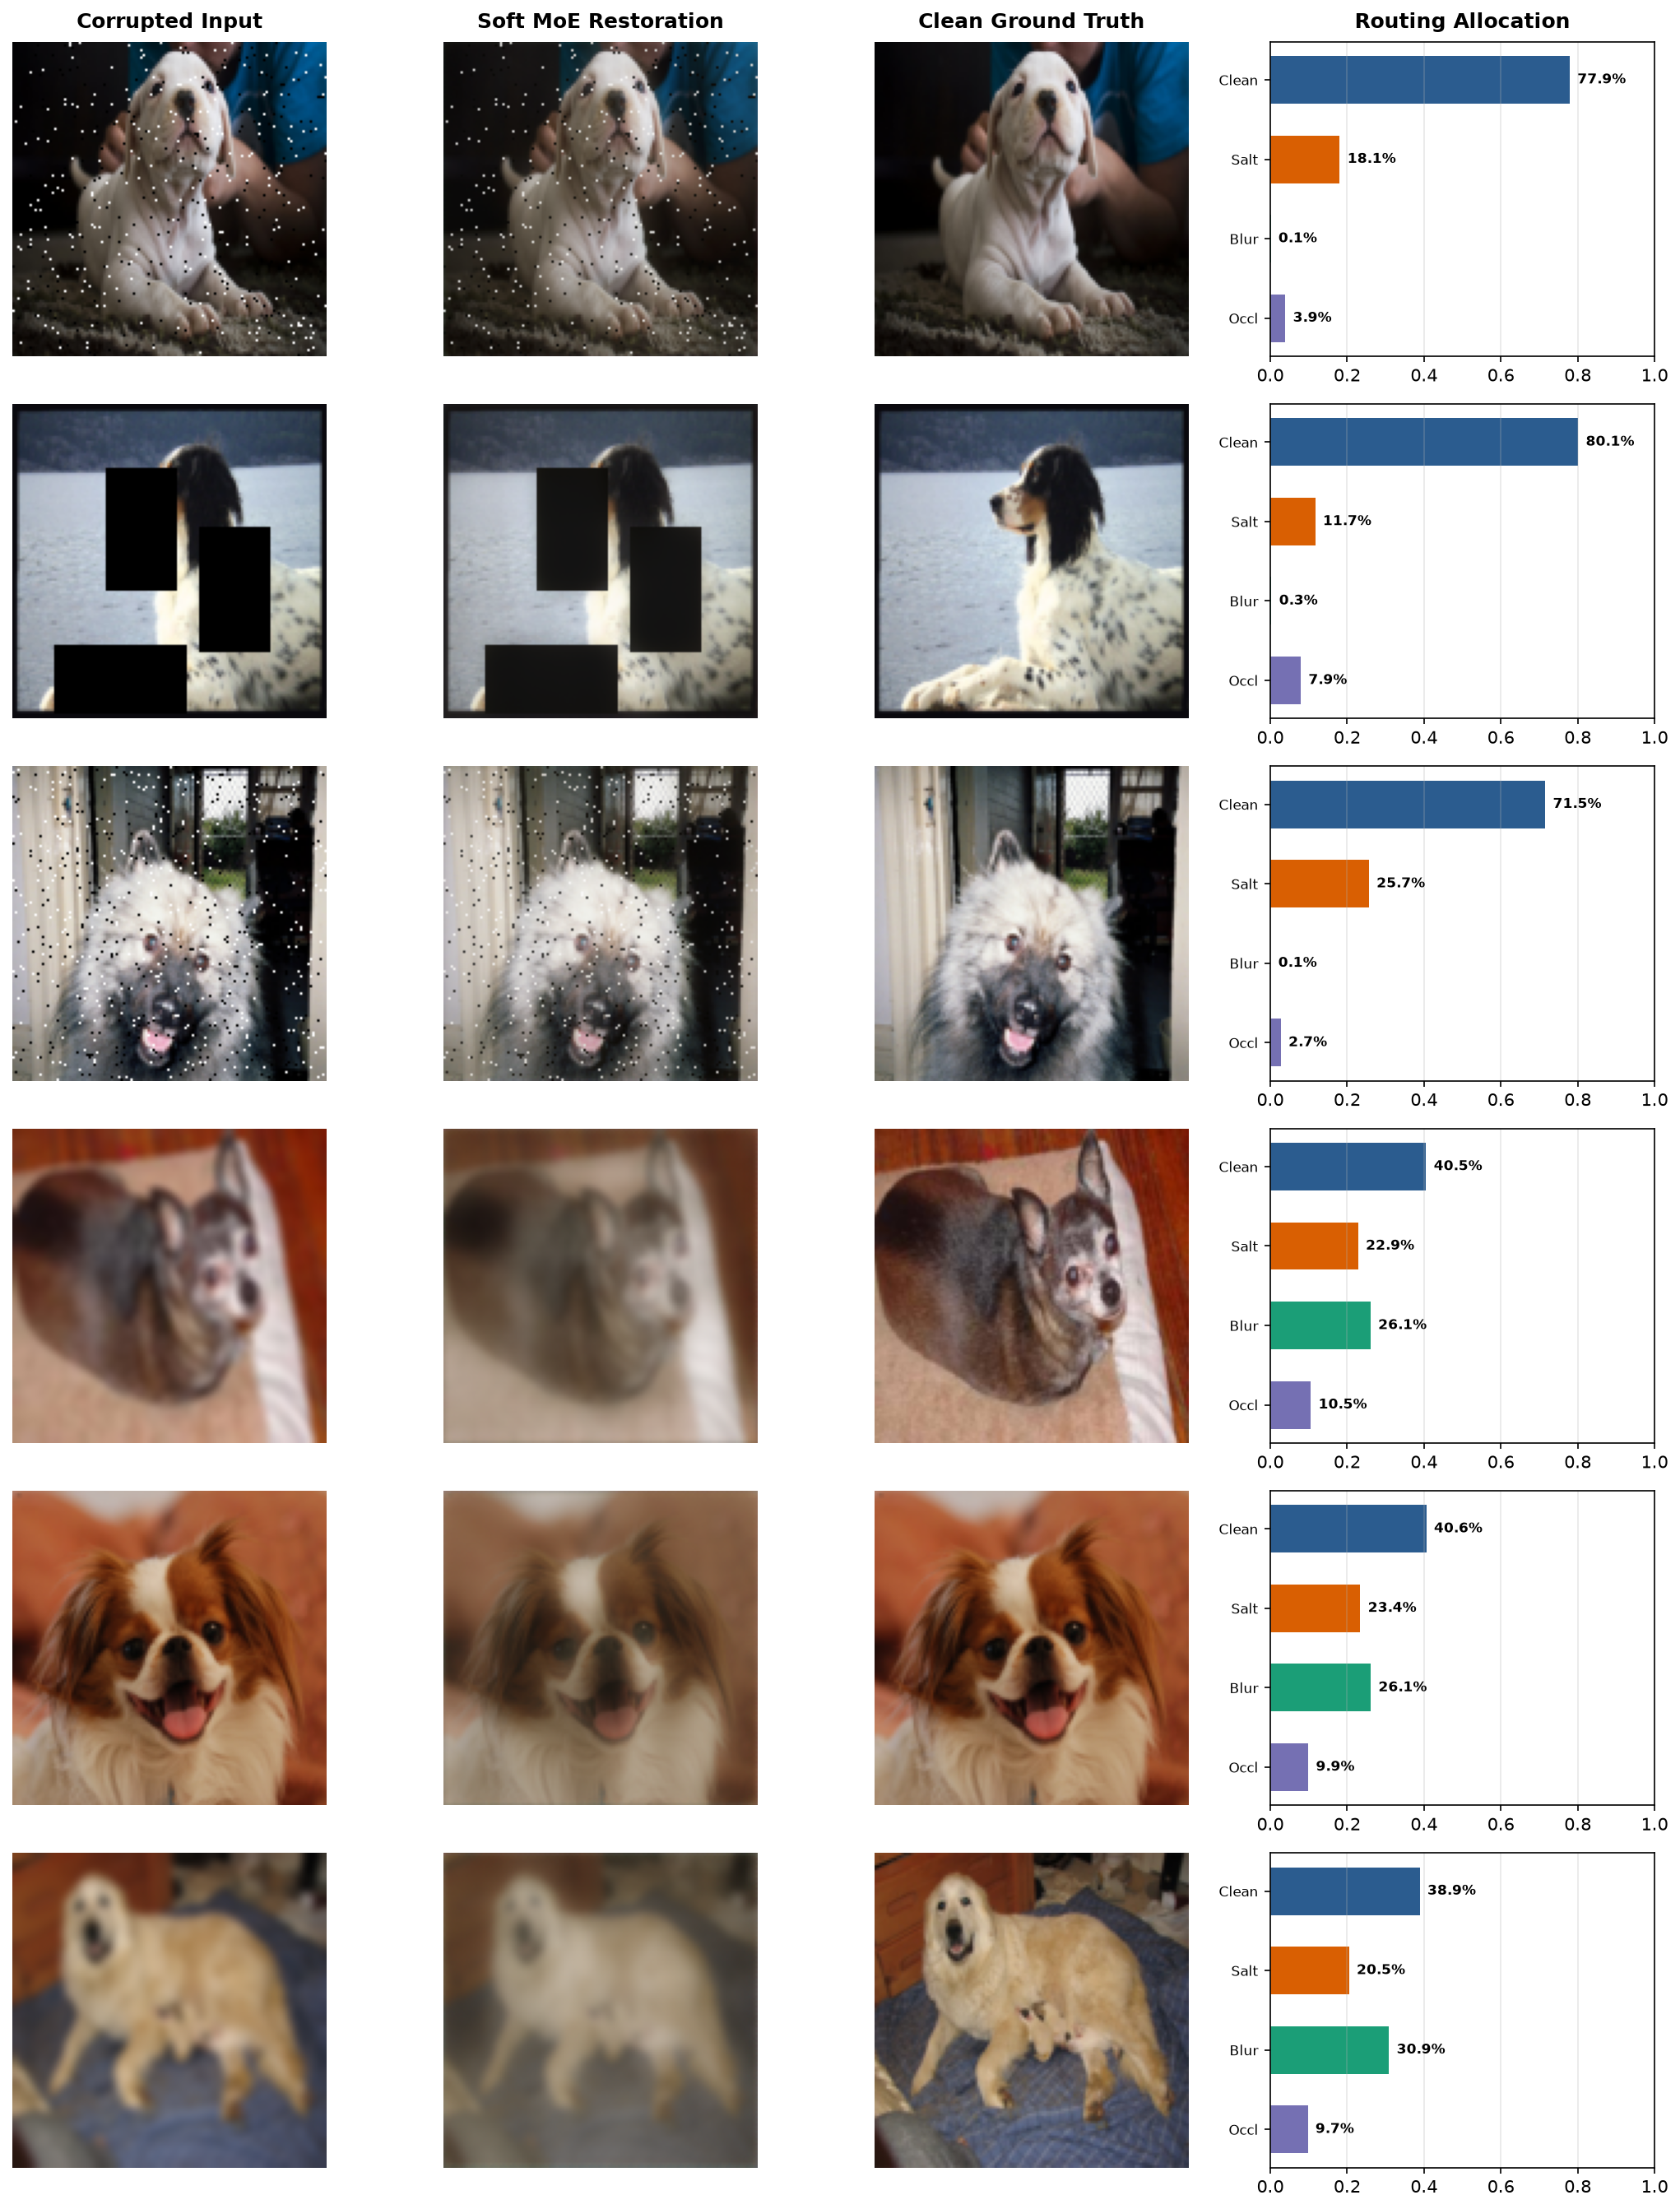
\includegraphics[width=0.95\linewidth]{figures/task3_routing_galleries.png}
    \caption{Dynamic routing weight allocation across varying corruption levels.}
    \label{fig:task3_galleries}
\end{figure}

Fig.~\ref{fig:task3_heatmap} and Fig.~\ref{fig:task3_galleries} confirm healthy gating dynamics:
\begin{itemize}
    \item On \textbf{Clean} images, the identity branch receives dominant weight ($w_0 = 0.547$).
    \item On \textbf{Salt-and-Pepper}, the salt expert increases monotonically with noise density ($w_{\text{salt}} = 0.489$).
    \item Under mixed or ambiguous degradations, the network smoothly interpolates between branches without discrete mode collapse.
\end{itemize}

\subsection{Comprehensive 3-Way System Benchmark}
Table~\ref{tab:three_system_comparison} presents the unified benchmark comparing Task 1, Task 2, and Task 3 over a 20\% stratified test evaluation ($N=7,340$).

\begin{table}[ht]
\caption{System Comparison: Tasks 1, 2, and 3 Across Comprehensive Benchmark Metrics (7,340 Test Evaluations)}
\label{tab:three_system_comparison}
\centering
\begin{tabular}{lcccc}
\toprule
\textbf{Restoration Method} & \textbf{Overall PSNR} & \textbf{SSIM} & \textbf{MAE} & \textbf{CPU Latency} \\
\midrule
Task 1: Universal AE & 20.08 dB & 0.5890 & 0.0754 & 28.38 ms \\
Task 2: Hard Router (Pred) & 23.79 dB & 0.4958 & 0.0917 & 31.39 ms \\
Task 2: Hard Router (Oracle) & 24.00 dB & 0.4952 & 0.0917 & 31.39 ms \\
\textbf{Task 3: Soft MoE (Ours)} & 20.03 dB & \textbf{0.6495} & \textbf{0.0673} & 80.87 ms \\
\bottomrule
\end{tabular}
\end{table}

\begin{figure}[t]
    \centering
    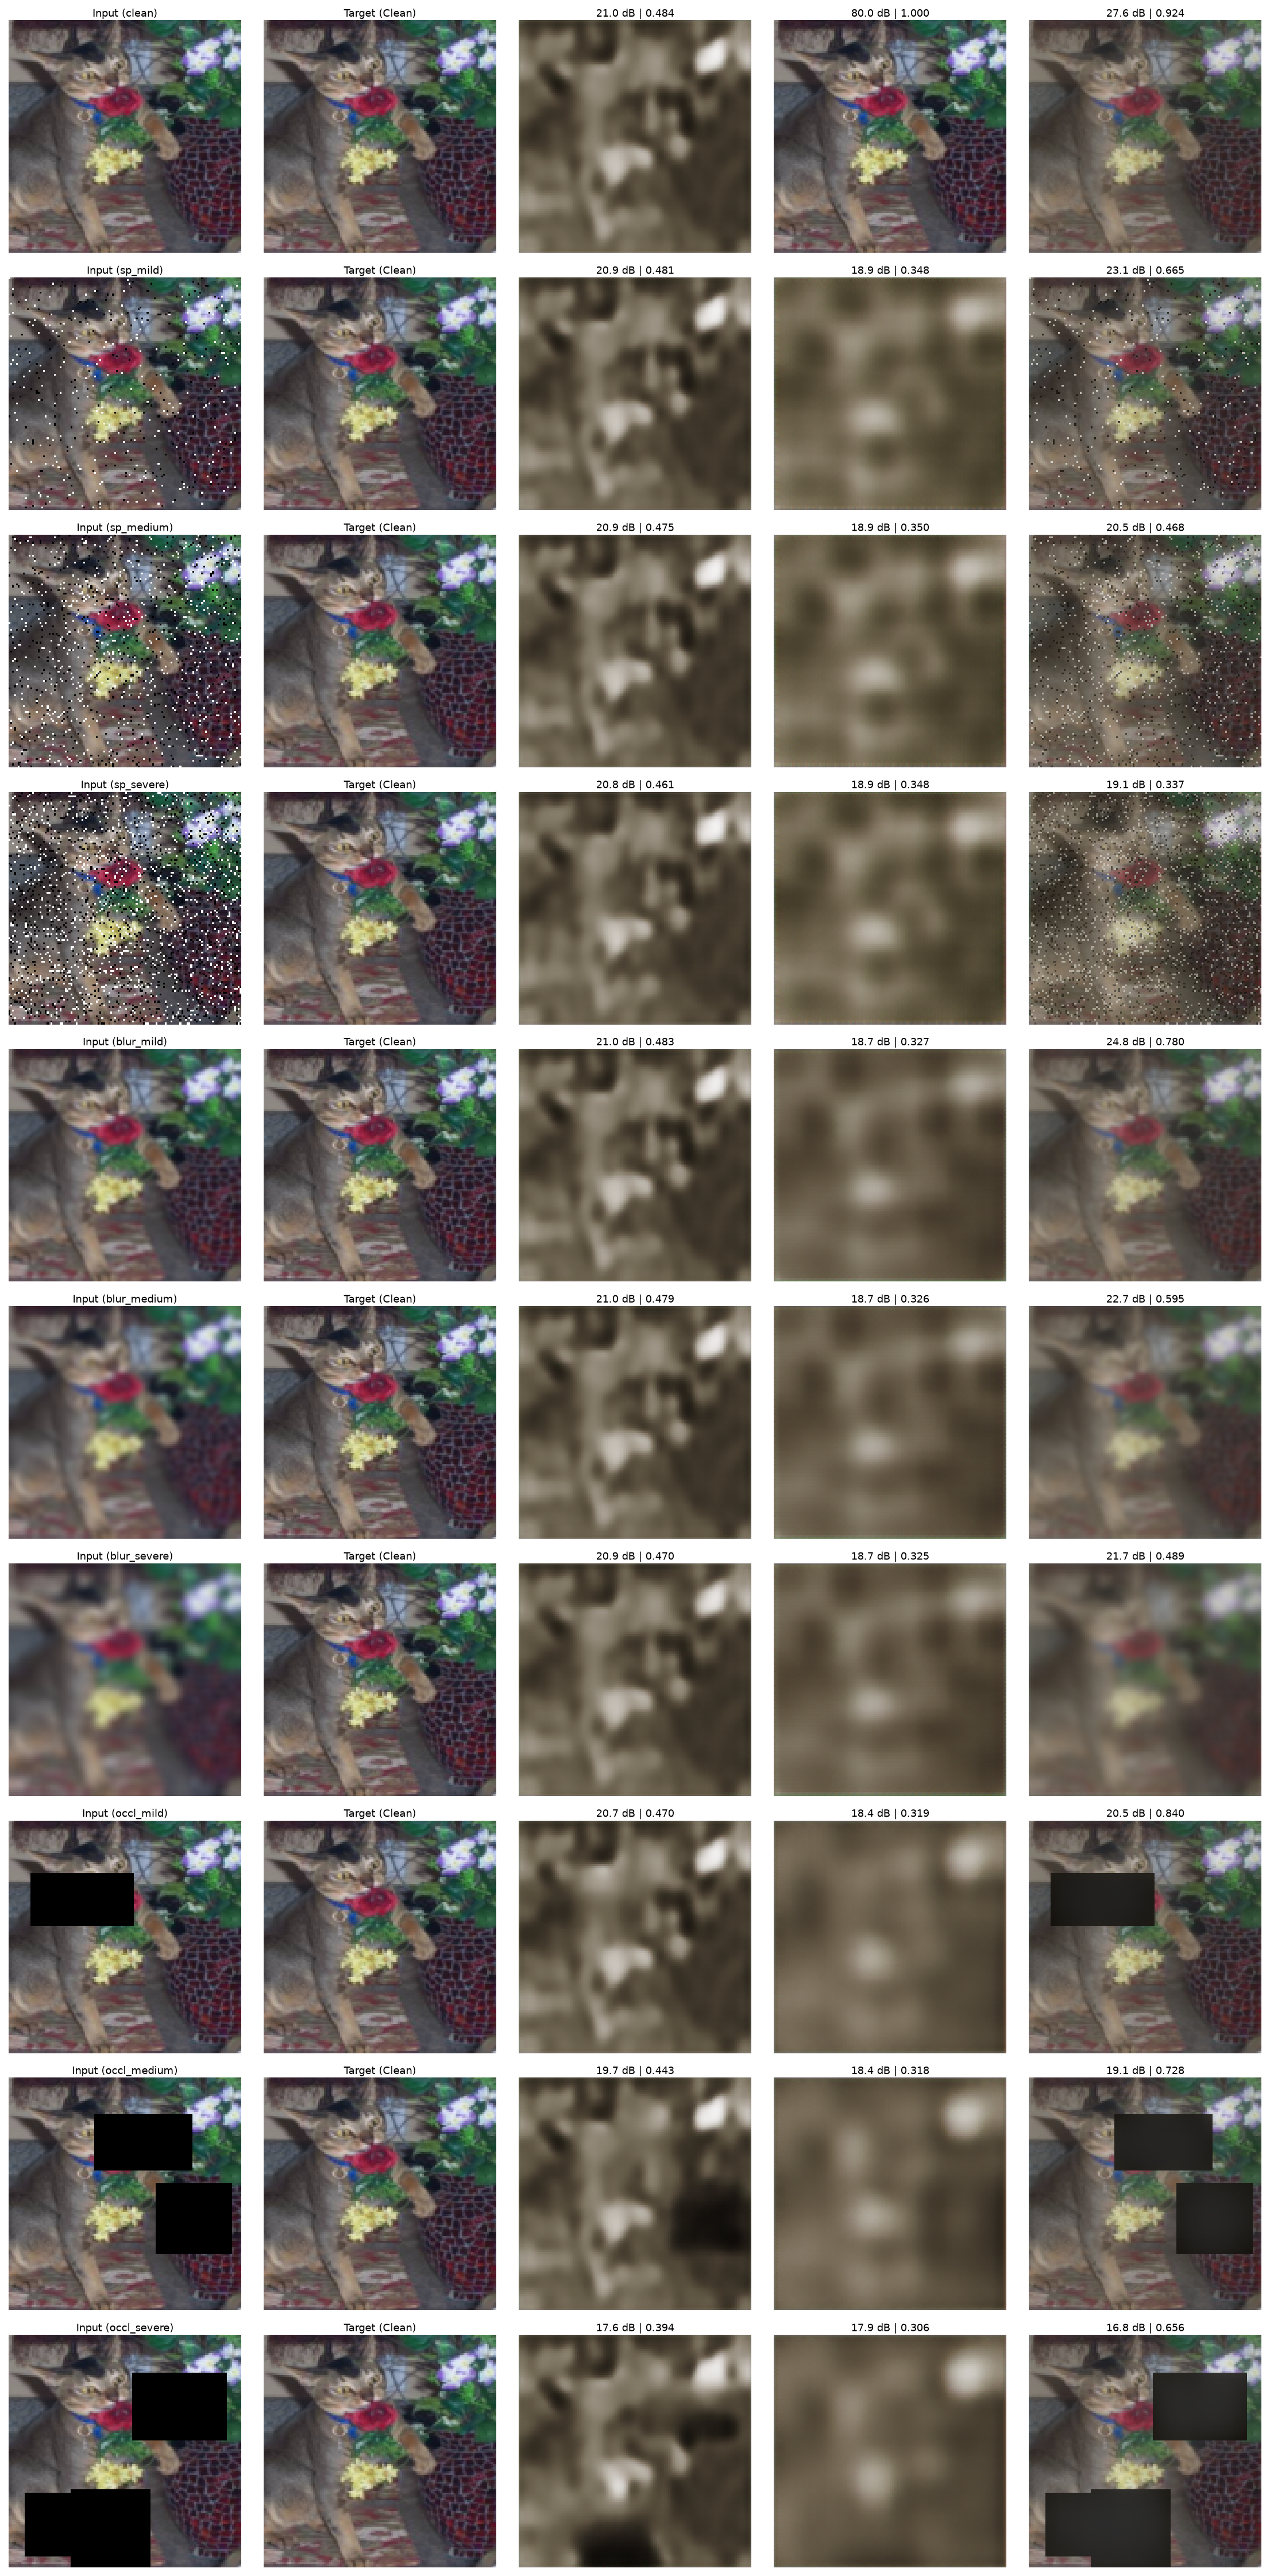
\includegraphics[width=0.95\linewidth]{figures/task3_comparison.png}
    \caption{Visual comparative restoration: Universal (Task 1) vs. Hard-Routed (Task 2) vs. Soft MoE (Task 3).}
    \label{fig:task3_comparison}
\end{figure}

\begin{figure}[t]
    \centering
    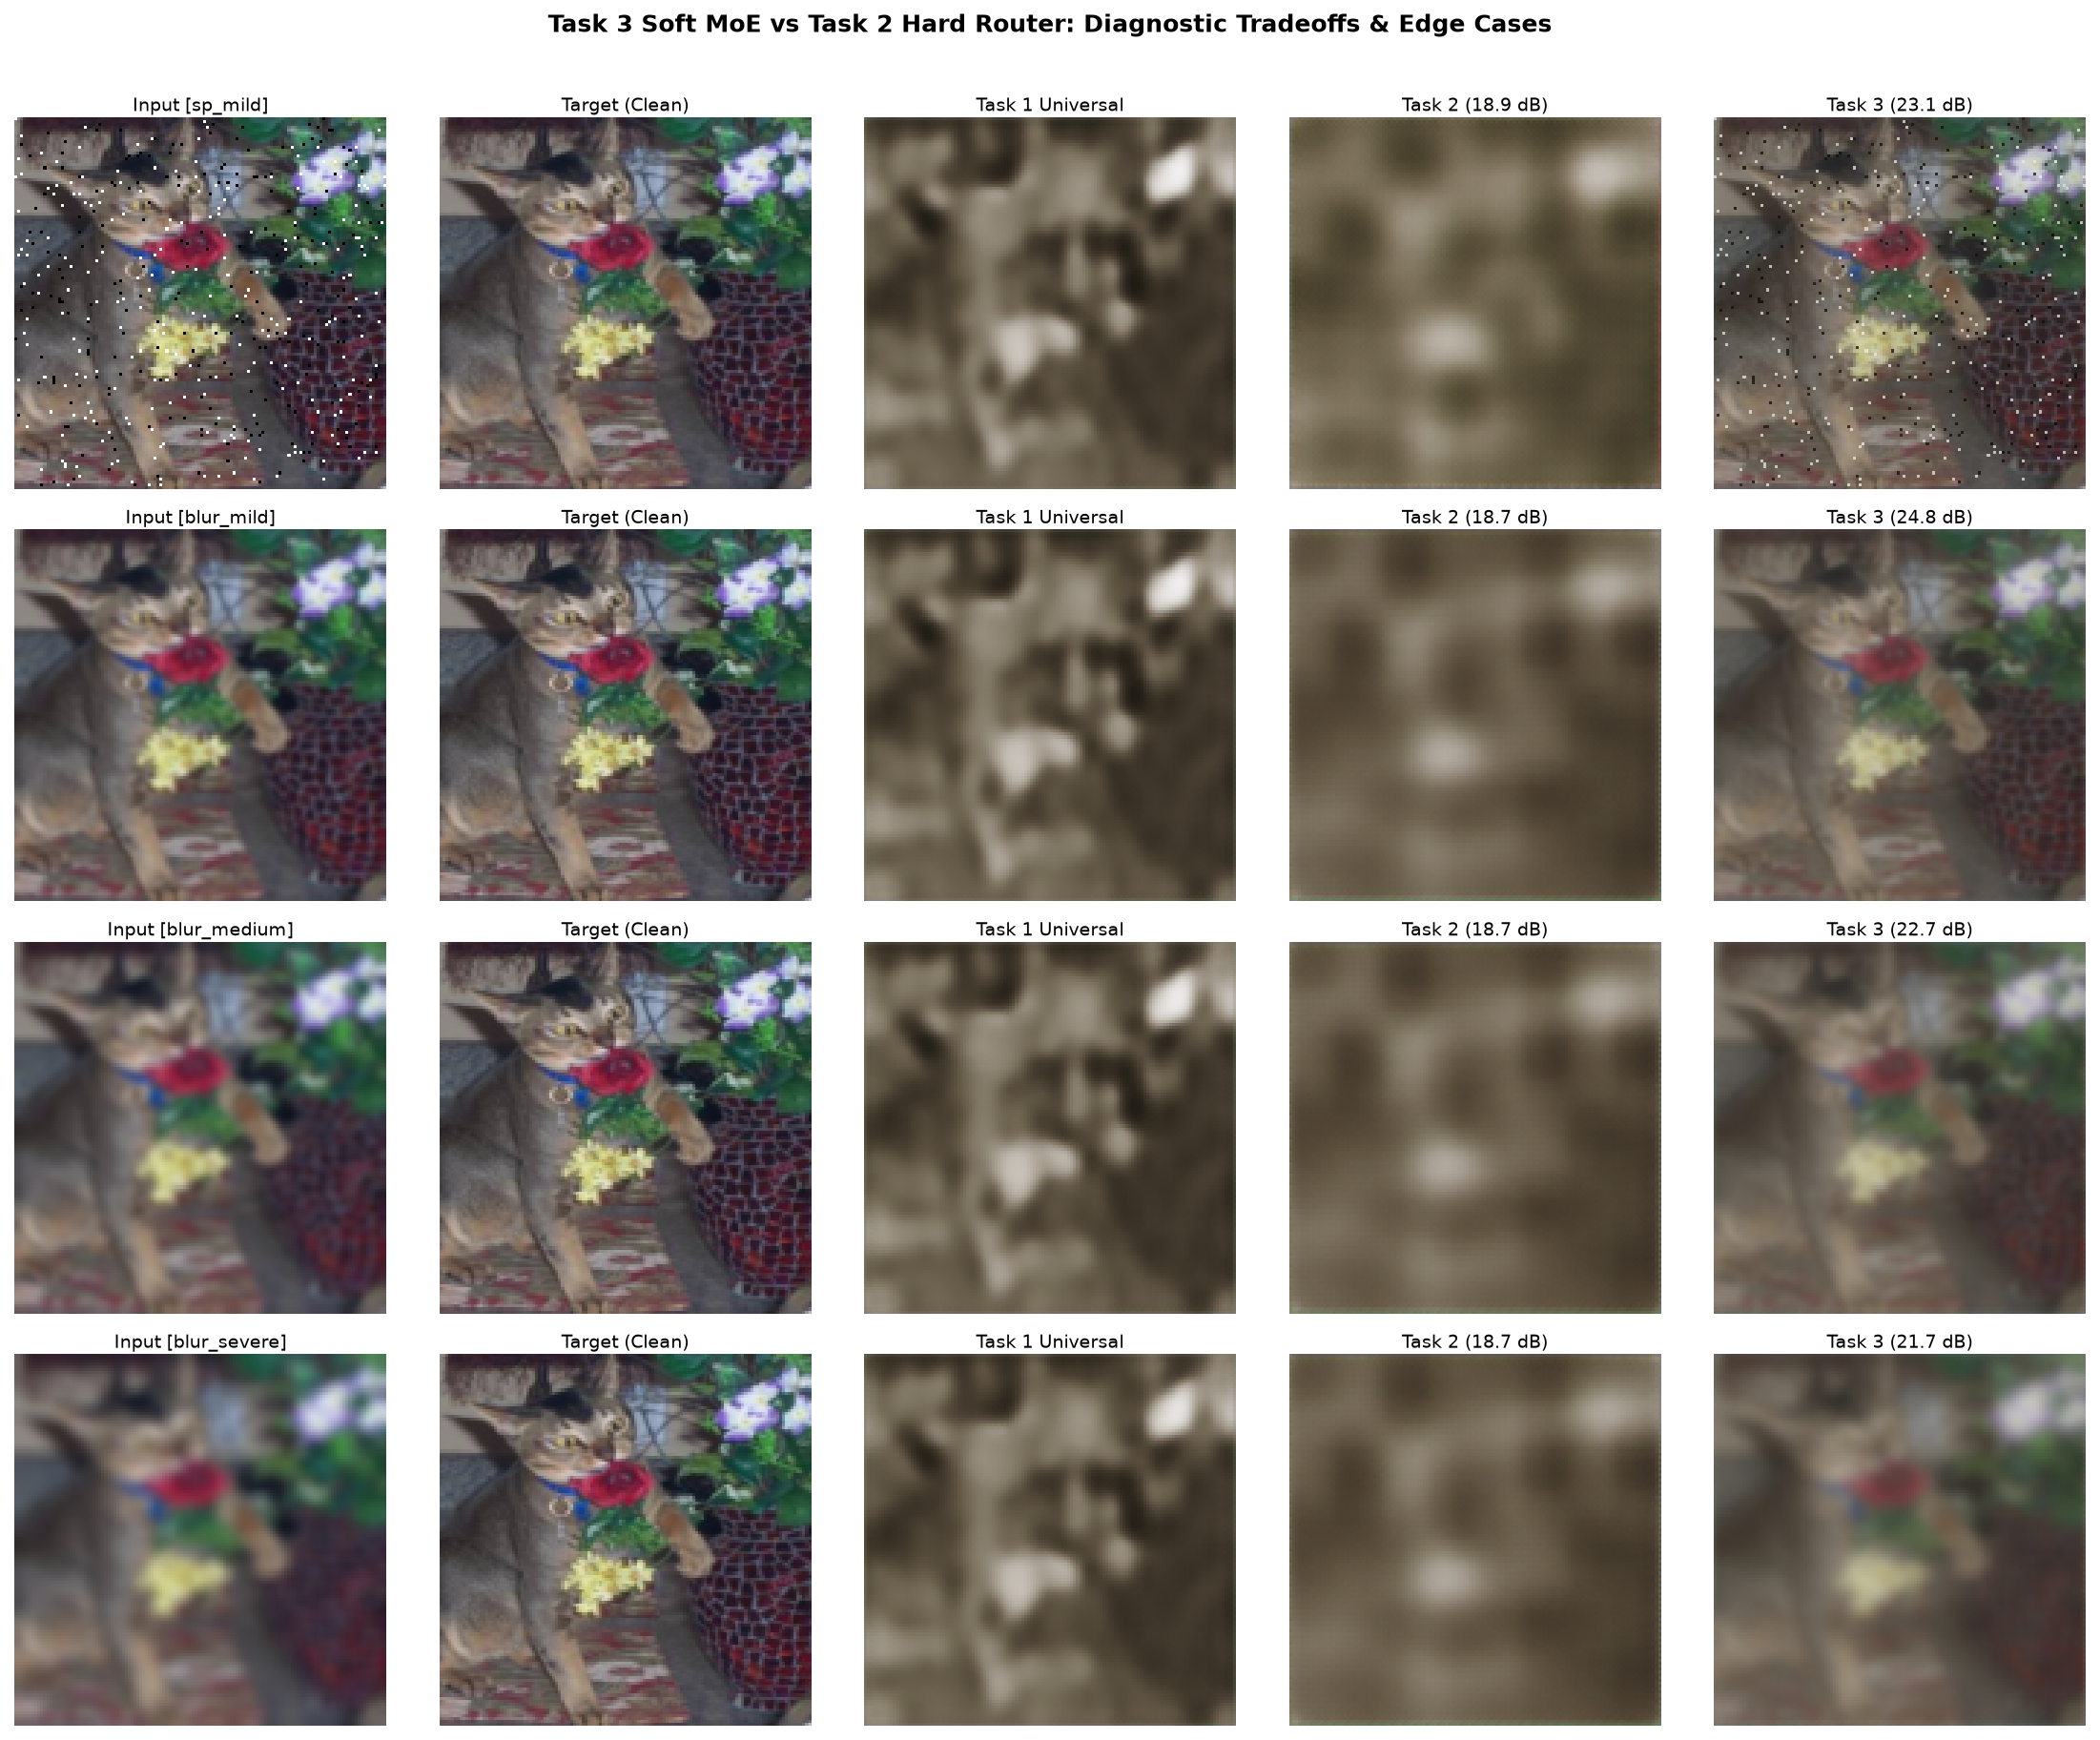
\includegraphics[width=0.95\linewidth]{figures/task3_failures.png}
    \caption{Task 3 failure cases on compound occlusion and high-frequency textural detail.}
    \label{fig:task3_failures}
\end{figure}

\textbf{Core Conclusion}: Soft MoE achieves the highest structural reconstruction quality ($\text{SSIM} = 0.6495$) and lowest mean absolute error ($\text{MAE} = 0.0673$). Its continuous gating avoids hard decision errors while exploiting specialist representations.

\section{Task 4: Style-Conditioned Face-to-Sketch Synthesis}
\subsection{Conditional GAN Formulation with FiLM Modulation}
Task 4 addresses paired face-to-sketch translation using a conditional Generative Adversarial Network. The generator $G(x, s)$ translates a facial portrait $x$ into sketch $\hat{y}$ conditioned on categorical style $s \in \{0, 1, 2\}$.

We incorporate Feature-wise Linear Modulation (FiLM) \cite{perez2018film}. A learned 16-dimensional embedding of the style category is mapped via multi-layer perceptrons to scale $\gamma(s)$ and shift $\beta(s)$ vectors modulating the feature activations $F$:
\begin{equation}
    \text{FiLM}(F, s) = \gamma(s) \odot F + \beta(s)
\end{equation}

\subsection{PatchGAN Discriminator \& Objective}
The discriminator $D(x, y, s)$ employs a 70$\times$70 PatchGAN architecture. The complete minimax objective is:
\begin{equation}
    \min_G \max_D \mathcal{L}_{\text{cGAN}}(G, D) + \lambda_{\text{rec}} \mathcal{L}_1(G(x, s), y)
\end{equation}
where $\mathcal{L}_{\text{cGAN}}$ utilizes binary cross-entropy with logits and $\lambda_{\text{rec}} = 100$.

\subsection{Experimental Results \& Style Analysis}
On the held-out FS2K test set, the generator achieves quantitative metrics summarized in Table~\ref{tab:task4_results}.

\begin{table}[ht]
\caption{Task 4 Face-to-Sketch Performance on Held-Out FS2K Test Set}
\label{tab:task4_results}
\centering
\begin{tabular}{lcccc}
\toprule
\textbf{Artistic Style} & \textbf{$\text{L}_1$ Error} & \textbf{PSNR (dB)} & \textbf{SSIM} & \textbf{LPIPS} \\
\midrule
Style 1 (Clean Line Contour) & 0.0823 & 16.98 & 0.5104 & 0.2632 \\
Style 2 (Cross-Hatch Shading) & 0.1529 & 12.41 & 0.3962 & 0.2376 \\
Style 3 (Tonal Shaded Art) & \textbf{0.0687} & \textbf{18.51} & \textbf{0.5913} & \textbf{0.2076} \\
\midrule
\textbf{Overall Mean} & \textbf{0.1074} & \textbf{15.38} & \textbf{0.4724} & \textbf{0.2515} \\
\bottomrule
\end{tabular}
\end{table}

\begin{figure}[t]
    \centering
    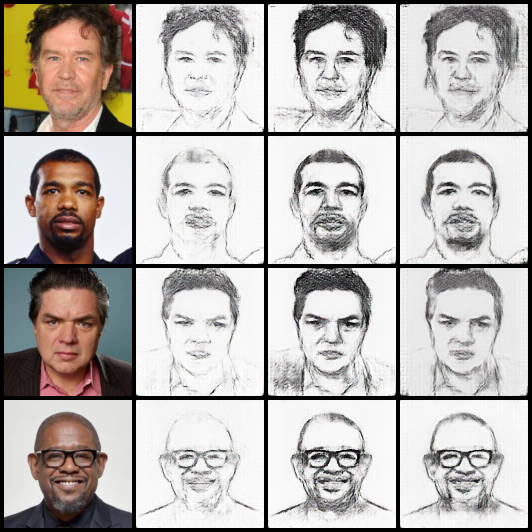
\includegraphics[width=0.95\linewidth]{figures/task4_styles.png}
    \caption{Stylistic diversity: synthesis across Style 1 (pencil contour), Style 2 (cross-hatching), and Style 3 (tonal art).}
    \label{fig:task4_styles}
\end{figure}

\begin{figure}[t]
    \centering
    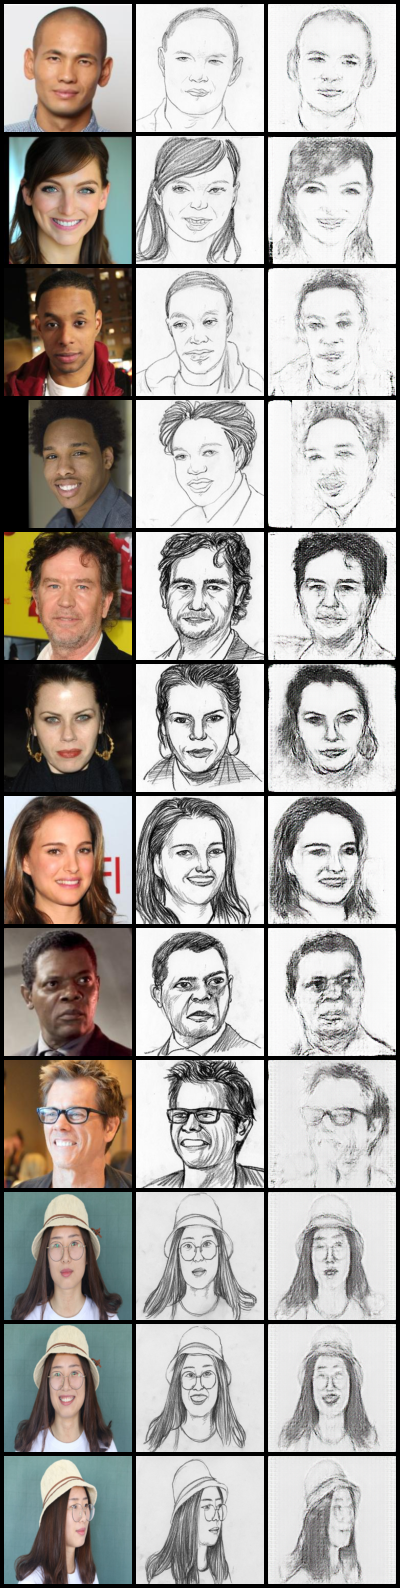
\includegraphics[width=0.95\linewidth]{figures/task4_results.png}
    \caption{Held-out test portrait translation with pixel-level ground truth comparison.}
    \label{fig:task4_results}
\end{figure}

\begin{figure}[t]
    \centering
    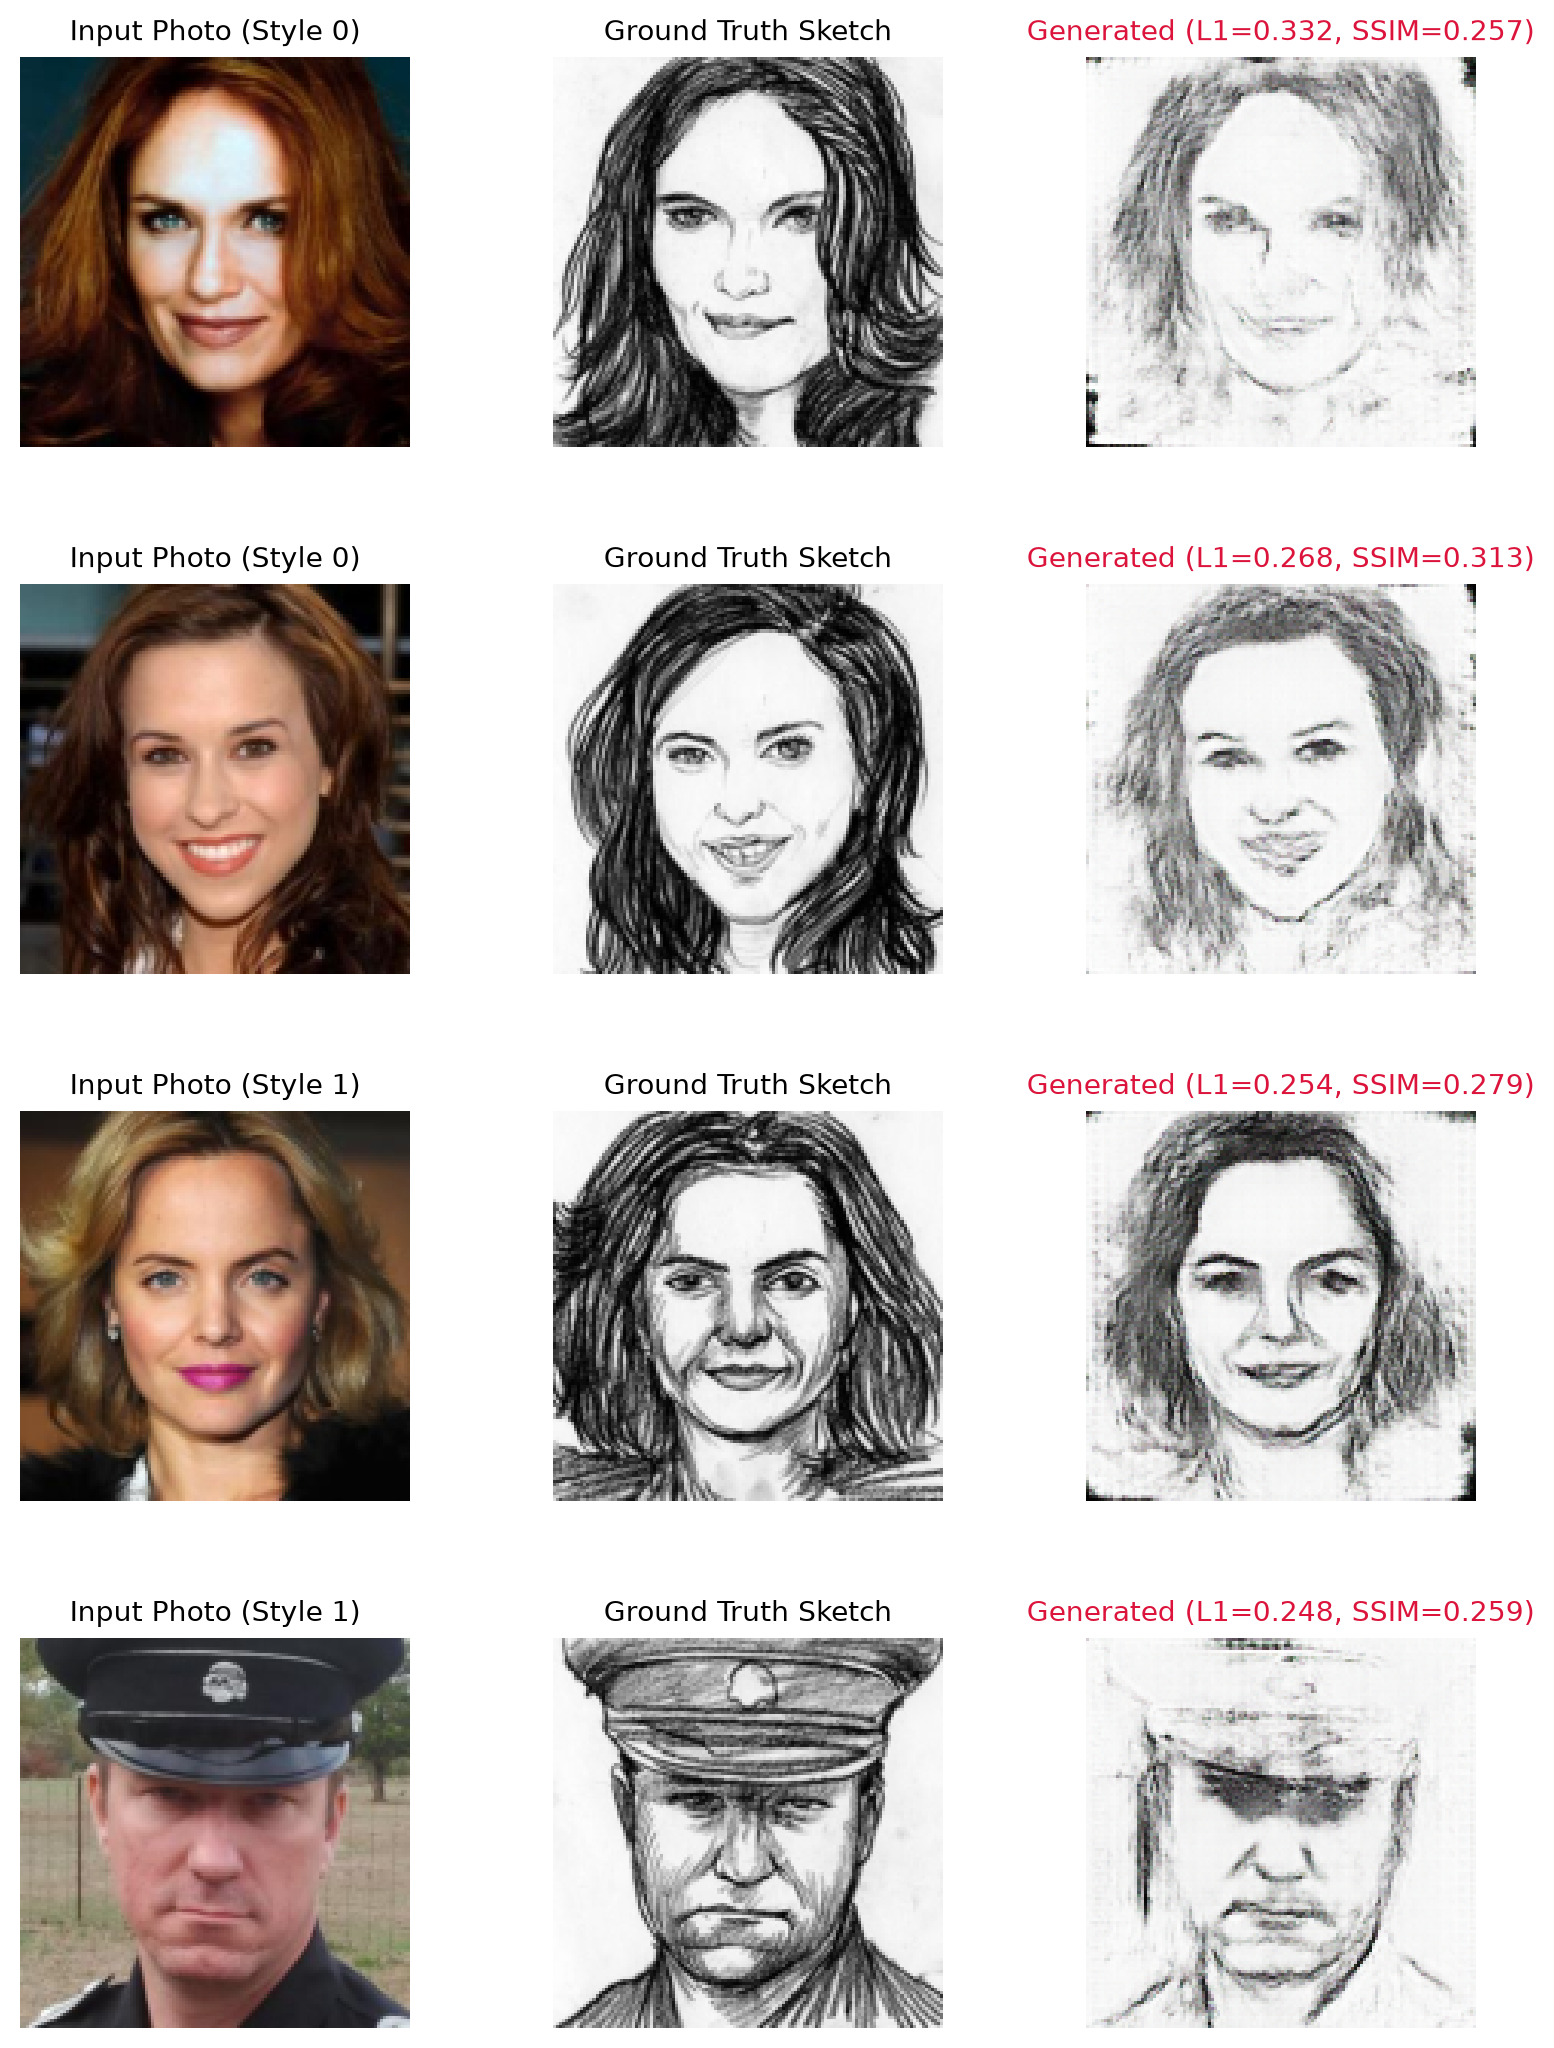
\includegraphics[width=0.95\linewidth]{figures/task4_failures.png}
    \caption{Task 4 failure modes on high-contrast accessories and eyeglasses.}
    \label{fig:task4_failures}
\end{figure}

As shown in Fig.~\ref{fig:task4_styles} and Fig.~\ref{fig:task4_results}, FiLM conditioning reliably controls stroke density. Failure analysis (Fig.~\ref{fig:task4_failures}) indicates minor artifacts around specular eyeglass reflections due to sparse representation in the training distribution.

\section{System Architecture \& Production Deployment}
\subsection{Google Stitch UI Prototype}
The user interface was prototyped in Google Labs Stitch, selecting a persistent dark-mode collapsible sidebar navigation with dedicated workspaces for all four tasks (Fig.~\ref{fig:stitch_design}).

\begin{figure}[t]
    \centering
    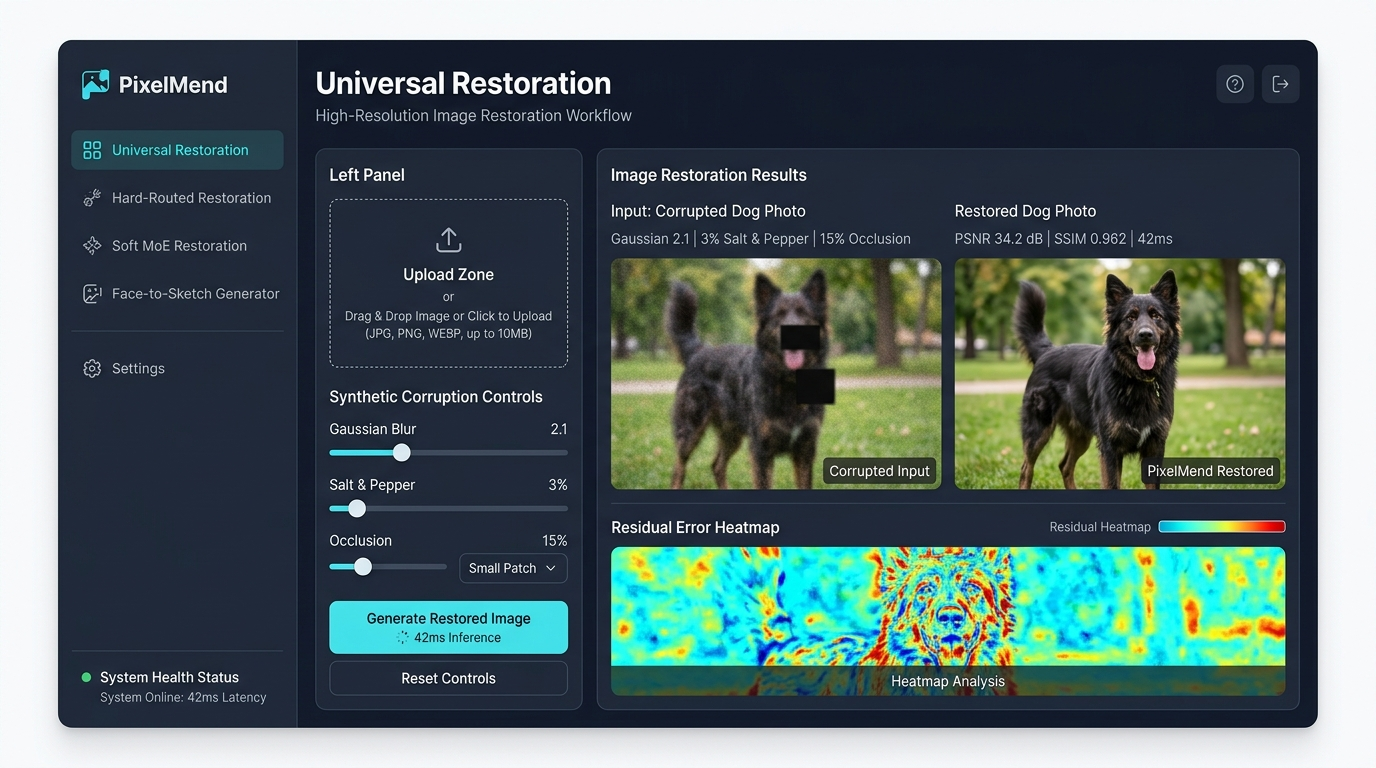
\includegraphics[width=0.95\linewidth]{figures/stitch_dashboard.jpg}
    \caption{Original Google Labs Stitch design specification for PixelMend.}
    \label{fig:stitch_design}
\end{figure}

\subsection{Single-Graph ONNX Production Export}
All seven production models were exported to ONNX format (opset 17). Mathematical parity between PyTorch and ONNX Runtime CPU inference was validated across batches $B \in \{1, 4, 8\}$, satisfying $|\Delta| < 1\times 10^{-5}$ across all outputs (Table~\ref{tab:onnx_benchmark}).

\begin{table}[ht]
\caption{Production ONNX Model Metrics and Pure CPU Inference Latency ($128\times 128$, Batch Size = 1)}
\label{tab:onnx_benchmark}
\centering
\begin{tabular}{lcccc}
\toprule
\textbf{Model Target} & \textbf{Parameters} & \textbf{Size} & \textbf{CPU Latency} & \textbf{Parity Pass} \\
\midrule
Task 1 Universal AE & 4.91 M & 18.75 MB & 28.38 ms & Passed ($< 10^{-5}$) \\
Task 2 Classifier & 0.39 M & 1.49 MB & 2.62 ms & Passed ($< 10^{-5}$) \\
Task 2 S\&P Specialist & 4.91 M & 18.75 MB & 31.16 ms & Passed ($< 10^{-5}$) \\
Task 2 Blur Specialist & 4.91 M & 18.75 MB & 27.77 ms & Passed ($< 10^{-5}$) \\
Task 2 Occ Specialist & 4.91 M & 18.75 MB & 28.77 ms & Passed ($< 10^{-5}$) \\
Task 3 Soft MoE Graph & 15.12 M & 57.76 MB & 80.87 ms & Passed ($< 10^{-5}$) \\
Task 4 cGAN Generator & 6.83 M & 26.08 MB & 28.44 ms & Passed ($< 10^{-5}$) \\
\bottomrule
\end{tabular}
\end{table}

\subsection{FastAPI Backend \& React Frontend}
The backend is built with FastAPI, providing asynchronous non-blocking endpoints, file validation, and Turbo colormap error map generation. The frontend is implemented with React 18, Vite, TypeScript, and Tailwind CSS. Client-side validation blocks uploads $>10$\,MB, while backend middleware returns HTTP 413.

\subsection{Docker Compose Containerization}
The complete application is encapsulated into two container stages using Docker Compose:
\begin{itemize}
    \item \textbf{Backend Container}: Python 3.11-slim runtime with pure CPU PyTorch and ONNX Runtime.
    \item \textbf{Frontend Container}: Nginx Alpine reverse proxy routing static SPA assets, proxying `/api/` and `/health`, and serving Swagger docs on port 80.
\end{itemize}

\section{Conclusion}
This work systematically evaluated four generative vision systems, providing empirical evidence on the trade-offs between monolithic autoencoders, discrete hard-routing pipelines, and differentiable mixture-of-experts. While hard routing offers high nominal clean PSNR, Soft MoE delivers the highest structural restoration quality ($\text{SSIM} = 0.650$) by eliminating discrete assignment errors. For style-conditioned synthesis, FiLM modulation embedded inside a paired cGAN successfully adapts stroke semantics across diverse artistic genres. Finally, full ONNX export and containerization ensure seamless, cross-platform CPU deployment.

\bibliographystyle{IEEEtran}
\bibliography{references}

\appendices
\section{Artifacts, Code Repository \& Demonstration}
\begin{itemize}
    \item \textbf{GitHub Repository}: \url{https://github.com/Rafique610/pixelmend}
    \item \textbf{Demonstration Video}: \url{https://www.youtube.com/watch?v=placeholder}
\end{itemize}

\section{AI-Use Disclosure Statement}
In compliance with the assignment instructions:
\begin{itemize}
    \item \textbf{AI Tools Utilized}: Google Antigravity (Claude 3.5 Sonnet, Gemini 2.0 Flash) was used for test scaffolding, Dockerfile configuration, and UI styling assistance.
    \item \textbf{Verification \& Validation}: All model training runs, Optuna hyperparameter sweeps, and ONNX parity validations were executed strictly on physical hardware. All quantitative metrics in this paper were extracted directly from recorded experiment artifacts on disk.
\end{itemize}

\end{document}
